\documentclass[sigconf,screen]{acmart}

\usepackage{microtype}
\usepackage{libertine}
\usepackage[T1]{fontenc}

\usepackage[normalem]{ulem}
\usepackage[bottom]{footmisc}

\usepackage{balance}
\usepackage{caption}
\usepackage{tightenum}

\usepackage{soul}
\usepackage[toc,page]{appendix}

\usepackage{subfig}


\usepackage{hyperref}
\hypersetup{hidelinks,colorlinks=true,linkcolor=red,citecolor=red}


\usepackage{setspace}
%\usepackage{epsf}
\usepackage{epsfig}
\usepackage{graphicx}
\usepackage{amsmath}
\usepackage{url}
\usepackage{nonfloat}
% % \urlstyle{rm}
% % {0em}{-0ex}{-2ex}

\usepackage{multirow}


% \usepackage{tikz}
% \usetikzlibrary{calc}
% \newcommand*\circled[1]{\tikz[baseline=-3pt]{
%             \node[shape=circle,draw,inner sep=1pt,minimum size=10pt] (char) {\small #1};}}

\usepackage{xcolor}
\definecolor{commentgreen}{RGB}{2,112,10}
\definecolor{eminence}{RGB}{108,48,130}
\definecolor{weborange}{RGB}{255,165,0}
\definecolor{frenchplum}{RGB}{129,20,83}

%
% Generic Defines
%

\newcommand{\mm}{mm$^2$}
\newcommand{\figtitle}[1]{\textbf{#1}}
\newcommand{\us}{$\mu$s}
\newcommand{\fixme}[1]{{\color{red}\textbf{\fbox{FIXME} #1}}}
\newcommand{\FIXME}[1]{{\color{red}\textbf{\fbox{FIXME} #1}}}
\newcommand{\TODO}[1]{{\color{red}\textbf{\fbox{TODO} #1}}}
\newcommand{\NOTE}[1]{{\color{blue}\textbf{\fbox{NOTE} #1}}}
\newcommand{\note}[1]{{\color{blue}\textbf{\fbox{NOTE} #1}}}

\newcommand{\yiying}[1]{{\color{cyan}\textbf{\fbox{Yiying} #1}}}
\newcommand{\arvind}[1]{{\color{orange}\textbf{\fbox{Arvind} #1}}}
\newcommand{\yizhou}[1]{{\color{red}\textbf{\fbox{Yizhou} #1}}}
\newcommand{\ryan}[1]{{\color{green}\textbf{\fbox{Ryan} #1}}}
\newcommand{\will}[1]{{\color{olive}\textbf{\fbox{Will} #1}}}
%\fbox{Zac} #1}}}

%\newcommand{\note}[2]{\fixme{$\ll$ #1 $\gg$ #2}}

\newcommand{\myitem}[1]{\item \textbf{#1}}
\newcommand{\myitemit}[1]{\item \textit{#1}}

\usepackage{listings}
\lstset {
    language=C,
    frame=tb,
    tabsize=2,
    showstringspaces=false,
    %numbers=left,
    %upquote=true,
    commentstyle=\color{commentgreen},
    keywordstyle=\color{eminence},
    stringstyle=\color{red},
    basicstyle=\scriptsize\ttfamily, % basic font setting
    emph={int,char,double,float,unsigned,void,bool},
    emphstyle={\color{blue}},
    otherkeywords={rread,rwrite,ralloc,ras_lock,rlock,runlock,rrelease,rpoll},
    keywordstyle={\color{purple}},
    escapechar=\&,
    % keyword highlighting
    classoffset=1, % starting new class
    %otherkeywords={>,<,.,;,-,!,=,~},
    %morekeywords={>,<,.,;,-,!,=,~},
    %keywordstyle=\color{weborange},
    classoffset=0,
}

\sloppy
\newcommand{\horizbar}{\rule{\linewidth}{.5mm}}
\newcommand{\app}[1]{{\sc #1}}
 
\renewcommand{\em}{\it}

  
\newcommand{\BigO}[1]{${\cal O}(#1)$}
\newcommand{\BigOmega}[1]{$\Omega(#1)$}
\newcommand{\BigTheta}[1]{$\Theta(#1)$}
 
\newcommand{\ceiling}[1]{\left\lceil #1 \right\rceil}
\newcommand{\faM}{\lfloor \alpha M \rfloor}
%\newcommand{\C}[2]{{#1 \choose #2}}

\newcommand{\x}{$\times$}
 
%\newcommand{\comment}[1]{}
\newcommand{\ignore}[1]{}


%\newcommand{\boldparagraph}[1]{\vspace*{-0ex}\paragraph{#1}}
\newcommand{\boldparagraph}[1]{\vspace*{1ex}\noindent\textit{#1}\hspace{1em}}

%%%%% SINGLE FIGURE
\def\cfigure[#1,#2,#3]{
\begin{figure}
\vspace*{0mm}
\begin{center}

\includegraphics[width=3in]{#1} 
 
\vspace*{-3mm}\caption[]{#2
} \label{#3}
 
\vspace*{-5mm}
\end{center}
%\horizbar
%\vspace*{-2mm}
\end{figure}}

%%%%% SINGLE FIGURE 4in wide
\def\cfigurefour[#1,#2,#3]{
\begin{figure}
\vspace*{0mm}
\begin{center}

\includegraphics[width=4in]{#1} 
 
\vspace*{-3mm}\caption[]{#2
} \label{#3}
 
\vspace*{-5mm}
\end{center}
%\horizbar
%\vspace*{-2mm}
\end{figure}}

%%%%% SINGLE FIGURE
\def\cfiguretemp[#1,#2,#3]{
\begin{figure}
\vspace*{0mm}
\begin{center}

\includegraphics[width=3.5in]{#1} 
 
\vspace*{-3mm}\caption[]{#2
} \label{#3}
 
\vspace*{-5mm}
\end{center}
%\horizbar
\vspace*{-2mm}
\end{figure}}

%%%%% SINGLE WIDE FIGURE
\def\wfigure[#1,#2,#3]{
\begin{figure*}
\vspace*{0mm}
\begin{center}
 \includegraphics[width=\textwidth]{#1} 
 \vspace*{-3mm}\caption[]{#2
} \label{#3}
 
\end{center}
%\horizbar
\end{figure*}}

%%%%% 3 FIGURES IN A ROW
\def\threefigure[#1,#2,#3,#4,#5]{
\begin{figure*}
\vspace*{0mm}
\begin{center}

\begin{tabular}{ccc}
\includegraphics[width=2in]{#1} & \includegraphics[width=2in]{#2} &  \includegraphics[width=2in]{#3} \\
(a) & (b) & (c) \\
\end{tabular}

\vspace*{-3mm}\caption[]{#4
} \label{#5}

\vspace*{-5mm}
\end{center}
%\horizbar
\vspace*{-2mm}
\end{figure*}}

%%%%%% DOUBLE FIGURE
\def\dcfigure[#1,#2,#3,#4,#5,#6]{
{
\begin{figure*}
\begin{center}
\begin{minipage}[c]{\columnwidth}{
\includegraphics[width=\columnwidth]{#1} 
\vspace*{0mm}\caption[]{#2} \label{#3} \
}\end{minipage}\hspace*{\columnsep}\
\begin{minipage}[c]{\columnwidth}{
\includegraphics[width=\columnwidth]{#4} 
\vspace*{0mm}\caption[]{#5}\label{#6} \
}\end{minipage}
\end{center}
\end{figure*}
}
}


\def\tableByTable[#1,#2,#3,#4,#5,#6]{
{
\begin{table*}
\begin{center}
\begin{minipage}[c]{3in}{
\centering
{#1}
\vspace*{0mm}\tabcaption[]{#2}\label{#3} \
}\end{minipage}\hspace*{\columnsep}\
\begin{minipage}[c]{3in}{
\centering
{#4}
\vspace*{0mm}\tabcaption[]{#5}\label{#6} \
}\end{minipage}
\end{center}
\end{table*}
}
}


\def\figureByTable[#1,#2,#3,#4,#5,#6]{
{
\begin{figure*}
\begin{center}
\begin{minipage}[c]{3in}{
\centering
\includegraphics[width=\textwidth]{#1}
\vspace*{0mm}\figcaption[]{#2} \label{#3} \
}\end{minipage}\hspace*{\columnsep}\
\begin{minipage}[c]{3.3in}{
\centering
{#4}
\vspace*{0mm}\tabcaption[]{#5}\label{#6} \
}\end{minipage}
\end{center}
\end{figure*}
}
}

\def\tableByFigure[#1,#2,#3,#4,#5,#6]{
{
\begin{figure*}
\begin{center}
\begin{minipage}[c]{4.3in}{
\centering
{#1}
\vspace*{0mm}\tabcaption[]{#2} \label{#3} \
}\end{minipage}\hspace*{\columnsep}\
\begin{minipage}[c]{2.2in}{
\centering
\includegraphics[width=\textwidth]{#4}
\vspace*{-0.35in}\caption[]{#5}\label{#6} \
}\end{minipage}
\end{center}
\end{figure*}
}
}

% two figs pdfs in one column fig
\def\doublecfigure[#1,#2,#3,#4]{
{
\begin{figure}
\begin{center}
\begin{minipage}[c]{1.5in}{
\begin{center}
\includegraphics[width=1.5in]{#1}%\\(a)
\end{center}
}\end{minipage}\hspace*{1em}\
\begin{minipage}[c]{1.5in}{
\begin{center}
\includegraphics[width=1.5in]{#2}%\\(b)
\end{center}
}\end{minipage}
\vspace*{0mm}\caption[]{#3} \label{#4} \
\end{center}
\end{figure}
}
}

\def\qcfigure[#1,#2,#3,#4,#5,#6]{
{
\begin{figure*}
\vspace*{0.2in}\
\begin{center}
\begin{minipage}[c]{3in}{
\includegraphics[width=3in]{#1} 
\vspace*{-3mm}
}
\end{minipage}\hspace*{0.5in}\
\begin{minipage}[c]{3in}{
\includegraphics[width=3in]{#2} 
\vspace*{-3mm}
}\end{minipage}

\begin{minipage}[c]{3in}{
\includegraphics[width=3in]{#3} 
\vspace*{-3mm}
}
\end{minipage}\hspace*{0.5in}\
\begin{minipage}[c]{3in}{
\includegraphics[width=3in]{#4} 
\vspace*{-3mm}
}\end{minipage}
\end{center}
\caption[]{#5}\label{#6}
\end{figure*}
}
}

\def\twfigure[#1,#2,#3,#4,#5]{
{
\begin{figure*}
\vspace*{0.2in}\
\begin{center}
\begin{minipage}[c]{6.5in}{
\includegraphics[width=6.5in]{#1} 
\vspace*{-3mm}
}
\end{minipage}

\begin{minipage}[c]{6.5in}{
\includegraphics[width=6.5in]{#2} 
\vspace*{-3mm}
}\end{minipage}

\begin{minipage}[c]{6.5in}{
\includegraphics[width=6.5in]{#3} 
\vspace*{-3mm}
}
\end{minipage}
\end{center}
\caption[]{#4}\label{#5}
\end{figure*}
}
}

\def\dwfigure[#1,#2,#3,#4]{
{
\begin{figure*}
\vspace*{0.2in}\
\begin{center}
\begin{minipage}[c]{6.5in}{
\includegraphics[width=6.5in]{#1} 
\vspace*{-3mm}
}
\end{minipage}

\begin{minipage}[c]{6.5in}{
\includegraphics[width=6.5in]{#2} 
\vspace*{-3mm}
}\end{minipage}

\end{center}
\caption[]{#3}\label{#4}
\end{figure*}
}
}



\def\dssfigure[#1,#2,#3,#4,#5,#6]{
{
\begin{figure*}
\vspace*{0.2in}\
\begin{center}
\begin{minipage}[c]{4in}{
\includegraphics[width=4in]{#1}
\vspace*{-3mm}\caption[]{#2} \label{#3} \
}\end{minipage}\hspace*{0.5in}\
\begin{minipage}[c]{2in}{
\includegraphics[width=2in]{#4}
\vspace*{-3mm}\caption[]{#5}\label{#6} \
}\end{minipage}
\end{center}
\vspace*{-0.4in}\
\end{figure*}
}
}




\def\dsfigure[#1,#2,#3,#4,#5,#6]{
{
\begin{figure*}
\vspace*{0.2in}\
\begin{center}
\begin{minipage}[c]{3in}{
\includegraphics[width=3in]{#1}
\vspace*{-3mm}\caption[]{#2} \label{#3} \
}\end{minipage}\hspace*{0.5in}\
\begin{minipage}[c]{3in}{
\hspace*{0.5in}\
\includegraphics[height=3in]{#4}
\vspace*{-3mm}\caption[]{#5}\label{#6} \
}\end{minipage}
\end{center}
\vspace*{-0.4in}\
\end{figure*}
}
}


\def\dsyfigure[#1,#2,#3,#4,#5,#6]{
{
\begin{figure*}
\vspace*{0.2in}\
\begin{center}
\begin{minipage}[c]{2.5in}{
\includegraphics[height=2.5in]{#1}
\vspace*{-3mm}\caption[]{#2} \label{#3} \
}\end{minipage}\hspace*{0.5in}\
\begin{minipage}[c]{2.5in}{
\includegraphics[height=2.5in]{#4}
\vspace*{-3mm}\caption[]{#5}\label{#6} \
}\end{minipage}
\end{center}
\vspace*{-0.4in}\
\end{figure*}
}
}

\def\dyfigure[#1,#2,#3,#4,#5,#6]{
{
\begin{figure*}
\vspace*{0.2in}\
\begin{center}
\begin{minipage}[c]{3in}{
\includegraphics[height=3in]{#1} 
\vspace*{-3mm}\caption[]{#2} \label{#3} \
}\end{minipage}\hspace*{0.5in}\
\begin{minipage}[c]{3in}{
\includegraphics[height=3in]{#4} 
\vspace*{-3mm}\caption[]{#5}\label{#6} \
}\end{minipage}
\end{center}
\vspace*{-0.4in}\
\end{figure*}
}
}

%%%%%% DOUBLE FIGURE Y
\def\dyoldfigure[#1,#2,#3,#4,#5,#6]{
{
\begin{figure*}
\vspace*{0.2in}\
\begin{center}
\begin{minipage}[c]{3in}{
\epsfysize=2.0in\
\hspace{0.5in}\
\epsfbox{#1}
\vspace*{-3mm}\caption[]{#2} \label{#3} \
}\end{minipage}\hspace*{0.25in}\
\begin{minipage}[c]{3in}{
\epsfysize=2.0in\
\hspace{0.5in}\
\epsfbox{#4}
\vspace*{-3mm}\caption[]{#5}\label{#6} \
}\end{minipage}
\end{center}
\vspace*{-0.4in}\
\end{figure*}
}
}

%%%%%% DOUBLE FIGURE Y IN A COLUMN!!
\def\cfiguredouble[#1,#2,#3,#4]{
\begin{figure}
\vspace*{0.2in}\
\begin{center}
\begin{minipage}[c]{1.5in}{
\epsfxsize=1.5in\
\epsfbox{#1}
}\end{minipage}\hspace*{0.1in}\
\begin{minipage}[c]{1.5in}{
\epsfxsize=1.5in\
\vspace{0.1in}\epsfbox{#2}
}\end{minipage}\vspace*{-0.10in} \caption[]{#3}\label{#4}
\end{center}
\vspace*{-0.4in}\
\end{figure}
}


%%%%% Single programmable size figure
\def\wpfigure[#1,#2,#3,#4]{
\begin{figure*}
\vspace*{4mm}
\begin{center}

\includegraphics[width=#4]{#1} 

\vspace*{-3mm}\caption[]{#2
} \label{#3}

\vspace*{-5mm}
\end{center}
%\horizbar
\end{figure*}}

%%%%% Single programmable size figure, rotated
\def\wprfigure[#1,#2,#3,#4,#5]{
\begin{figure*}
\vspace*{4mm}
\begin{center}

\includegraphics[width=#4, angle=#5]{#1} 

\vspace*{-3mm}\caption[]{#2
} \label{#3}

\vspace*{-5mm}
\end{center}
%\horizbar
\end{figure*}}




%%%%% Adjacent, programmable-width figures, slid vertically by 9th
%%%%% parameter
\def\DoubleFigureWSlide[#1,#2,#3,#4,#5,#6,#7,#8,#9]{
\begin{figure*}
\vspace*{#9}
\begin{center}
\begin{minipage}{#4}
\includegraphics[width=#4]{#1}
\vspace*{-3mm}\caption{#2
}\label{#3}
\end{minipage}
\hspace{2em}
\begin{minipage}{#8}
\includegraphics[width=#8]{#5}
\vspace*{-3mm}\caption{#6
}\label{#7}
\end{minipage}
\vspace*{-5mm}
\end{center}
\end{figure*}
}


%%%%% Adjacent, programmable-width figures
\def\DoubleFigureW[#1,#2,#3,#4,#5,#6,#7,#8]{
\begin{figure*}
\vspace*{0in}
\begin{center}
\begin{minipage}{#4}
\includegraphics[width=#4]{#1}
\vspace*{-3mm}\caption{#2
}\label{#3}
\end{minipage}
\hspace{2em}
\begin{minipage}{#8}
\includegraphics[width=#8]{#5}
\vspace*{-3mm}\caption{#6
}\label{#7}
\end{minipage}
\vspace*{-5mm}
\end{center}
\end{figure*}
}



\def\DoubleFigureWHack[#1,#2,#3,#4,#5,#6,#7,#8]{
\begin{figure*}
\vspace*{0in}
\begin{center}
\begin{minipage}{3in}
\includegraphics[width=#4]{#1}
\vspace*{-3mm}\caption{#2
}\label{#3}
\end{minipage}
\hspace{2em}
\begin{minipage}{3in}
\includegraphics[width=#8]{#5}
\vspace*{-3mm}\caption{#6
}\label{#7}
\end{minipage}
\vspace*{-5mm}
\end{center}
\end{figure*}
}






%%%%%% DOUBLE FIGURE
\def\ddcfigure[#1,#2,#3,#4]{
\begin{figure*}
\vspace*{0.2in}\
\begin{center}
\begin{minipage}[c]{\columnwidth}{
\includegraphics[width=\columnwidth]{#1} 
}\end{minipage}\hspace{0.5in}\
\begin{minipage}[c]{\columnwidth}{
\includegraphics[width=\columnwidth]{#2} 
}\end{minipage} \caption[]{#3}\label{#4}
\end{center}
\end{figure*}
}

\def\ddcfigureSlide[#1,#2,#3,#4,#5]{
\begin{figure*}
\vspace*{#5}\
\begin{center}
\begin{minipage}[c]{3in}{
\includegraphics[height=3in]{#1} 
}\end{minipage}\hspace{0.5in}\
\begin{minipage}[c]{3in}{
\includegraphics[height=3in]{#2} 
}\end{minipage}\vspace*{-0.10in} \caption[]{#3}\label{#4}
\end{center}
\vspace*{-0.4in}\
\end{figure*}
}

\def\cxfigure[#1,#2,#3]{
\begin{figure}
\vspace*{4mm}
\begin{center}
 
\epsfxsize=2.5in\
\epsfbox{#1}\
 
\vspace*{-0.10in}\caption[]{#2
} \label{#3}
 
\vspace*{-5mm}
\end{center}
%\horizbar
\vspace*{-2mm}
\end{figure}}

\newenvironment{panefigure}{\begin{figure}\begin{center}}{\end{center}\end{figure}}

\newcommand{\pdfpane}[3]{
\begin{minipage}{#1}
\begin{center}
\includegraphics[width=#1]{#2}\\(#3)
\end{center}
\end{minipage}
}

\newcommand{\figWidth}{\columnwidth}
\newcommand{\figSep}{0.05in} 
%\newcommand{\figSep}{\columnsep} 
\newcommand{\figWidthOne}{3.05in} 
\newcommand{\figWidthHalf}{5.85in} 
\newcommand{\figWidthTwo}{3.7in} 
\newcommand{\figWidthThree}{2in} 
\newcommand{\figWidthFour}{1.3in} 
\newcommand{\figWidthFive}{2.3in} 
\newcommand{\figWidthSix}{2.3in} 
\newcommand{\figHeight}{2.0in}
\newcommand{\figHeightOne}{2.6in}
\newcommand{\captionText}[2]{\textbf{#1} \textit{\small{#2}}}

\newcommand{\beforecaption}{\vspace{-.15cm}\begin{spacing}{0.85}}
\newcommand{\aftercaption}{\vspace{-.45cm}\end{spacing}}
% \newcommand{\mycaption}[3]{{\beforecaption\caption{\label{#1}\footnotesize{\textbf{#2}} {\em #3}}\aftercaption}}
% haryadi, change mycaption three to mycaptionthree
%\newcommand{\mycaption}[3]{{\caption[#2]{{\bf #2.} {\em #3}}\label{#1}}}
%\newcommand{\mycaption}[3]{\beforecaption\caption{\label{#1}{\small \bf #2} \em\scriptsize #3}\aftercaption}
%\newcommand{\mycaption}[3]{\beforecaption\caption{\label{#1}{\bf #2} \em\footnotesize #3}\aftercaption}
\newcommand{\mycaption}[3]{\caption{\label{#1}{\bf #2} \em\small #3}}


%%%%% general

% only foreign words should be italicized... (example given should not)
\newcommand{\eg}{\textit{e.g.}}
\newcommand{\ie}{\textit{i.e.}}
\newcommand{\etal}{\textit{et al.}}
\newcommand{\etc}{\textit{etc.}}
\newcommand{\adhoc}{\textit{ad hoc}}

% units
\newcommand{\KB}{\,KB}
\newcommand{\MB}{\,MB}
\newcommand{\GB}{\,GB}
\newcommand{\TB}{\,TB}
\newcommand{\GBs}{\,GB/s}
\newcommand{\MBs}{\,MB/s}
\newcommand{\KBs}{\,KB/s}
\newcommand{\Kbs}{~Kbit/s}
\newcommand{\gbps}{\,Gbps}
\newcommand{\mbs}{~Mbit/s}
\newcommand{\mus}{\mbox{$\mu s$}}
\newcommand{\ms}{\mbox{$ms$}}

%\newcommand{\fsync}{\texttt{fsync}}

% axes
\newcommand{\xaxis}{x-axis}
\newcommand{\yaxis}{y-axis}


\newcommand{\unix}{{\sc Unix}}
\newcommand{\NULL}{{\sc NULL}}
\newcommand{\sysread}{\texttt{read}}
\newcommand{\syssync}{\texttt{sync}}
\newcommand{\fsync}{\texttt{fsync}}
\newcommand{\syswrite}{\texttt{write}}
\newcommand{\sysseek}{\texttt{lseek}}
\newcommand{\sysstat}{\texttt{stat}}
\newcommand{\make}{\texttt{make}}
\newcommand{\ioctl}{\texttt{ioctl}}
\newcommand{\panic}{\texttt{panic}}
\newcommand{\truncate}{\texttt{truncate}}
\newcommand{\rmdir}{\texttt{rmdir}}
\newcommand{\unlink}{\texttt{unlink}}
\newcommand{\open}{\textit{open}}
\newcommand{\close}{\textit{close}}
\newcommand{\linkscount}{\texttt{linkscount}}
\newcommand{\msync}{\textit{msync}}
\newcommand{\mmap}{\textit{mmap}}
\newcommand{\unmap}{\textit{munmap}}
\newcommand{\map}{\textit{map}}
\newcommand{\fetch}{\textit{gfetch}}
\newcommand{\acquire}{\textit{acquire}}
\newcommand{\commitxact}{\textit{commit}}
\newcommand{\commit}{\textit{commit}}
\newcommand{\barrier}{\textit{thread-barrier}}


% dsnvm
\newcommand{\dsnvm}{DSPM}
\newcommand{\dsm}{DSM}
\newcommand{\nvm}{PM}
\newcommand{\hotpot}{Hotpot}
\newcommand{\mrmw}{MRMW}
\newcommand{\mrsw}{MRSW}
\newcommand{\wfetch}{FETCH}
\newcommand{\cd}{CD}
\newcommand{\dr}{DR}
\newcommand{\on}{ON}
\newcommand{\dn}{DN}
\newcommand{\xn}{CN}
\newcommand{\master}{MN}
\newcommand{\xactid}{CID}
\newcommand{\dirty}{dirty}
\newcommand{\committed}{committed}
\newcommand{\redundant}{redundant}
\newcommand{\ib}{IB}
\newcommand{\sendreply}{\texttt{send-reply}}
\newcommand{\atomicsendreply}{\texttt{atomic-send-reply}}
\newcommand{\multisendreply}{\texttt{multicast-send-reply}}
\newcommand{\journaled}{JOURNALED}
\newcommand{\fsyncsafe}{FSYNC\_SAFE}
\newcommand{\X}{{$\times$}}
\newcommand{\pmfs}{PMFS}
\newcommand{\tmpfs}{tmpfs}
\newcommand{\Octopus}{Octopus}
\newcommand{\Mojim}{Mojim}
\newcommand{\dsmnoxact}{DSM-NoXact}
\newcommand{\dsmxact}{DSM-Xact}
\newcommand{\clflush}{\texttt{clflush}}
\newcommand{\pcommit}{\texttt{pcommit}}
\newcommand{\mfence}{\texttt{mfence}}
\newcommand{\sfence}{\texttt{sfence}}
\newcommand{\ra}{\textbf{R1.a}}
\newcommand{\rb}{\textbf{R1.b}}
\newcommand{\rcs}{\textbf{R2.a}}
\newcommand{\rcm}{\textbf{R2.b}}
\newcommand{\rdr}{\textbf{R3.r}}
\newcommand{\rdu}{\textbf{R3.u}}
\newcommand{\re}{\textbf{R3}}
\newcommand{\rf}{\textbf{R4}}

%\newcommand{\ignore}[1]{}
\input{remark}
%% Leave this on, so we can see them!!!
\remarktrue
\newcommand{\shortenum}{\vspace*{-0.1in}}
\newcommand{\sparagraph}[1]{\vspace*{0.0in}\paragraph{#1}}

% add below for confidential distribution
%\usepackage{draftwatermark}
%\SetWatermarkText{DO NOT DISTRIBUTE}
%\SetWatermarkScale{0.4}

%%% If you see 'ACMUNKNOWN' in the 'setcopyright' statement below,
%%% please first submit your publishing-rights agreement with ACM (follow link on submission page).
%%% Then please update our instructions page and copy-and-paste the NEW commands into your article.
%%% Please contact us in case of questions; allow up to 10 min for the system to propagate the information.
%%%
%%% The following is specific to ASPLOS '22 and the paper
%%% 'Clio: A Hardware-Software Co-Designed Disaggregated Memory System'
%%% by Zhiyuan Guo, Yizhou Shan, Xuhao Luo, Yutong Huang, and Yiying Zhang.
%%%

\setcopyright{rightsretained}
\acmPrice{}
\acmDOI{10.1145/3503222.3507762}
\acmYear{2022}
\copyrightyear{2022}
\acmSubmissionID{asplos22main-p968-p}
\acmISBN{978-1-4503-9205-1/22/02}
\acmConference[ASPLOS '22]{Proceedings of the 27th ACM International Conference on Architectural Support for Programming Languages and Operating Systems}{February 28 -- March 4, 2022}{Lausanne, Switzerland}
\acmBooktitle{Proceedings of the 27th ACM International Conference on Architectural Support for Programming Languages and Operating Systems (ASPLOS '22), February 28 -- March 4, 2022, Lausanne, Switzerland}
\keywords{Resource Disaggregation, FPGA, Virtual Memory, Hardware-Software Co-design}
\begin{CCSXML}
<ccs2012>
<concept>
<concept_id>10010520.10010521.10010537.10003100</concept_id>
<concept_desc>Computer systems organization~Cloud computing</concept_desc>
<concept_significance>500</concept_significance>
</concept>
<concept>
<concept_id>10010583.10010588</concept_id>
<concept_desc>Hardware~Communication hardware, interfaces and storage</concept_desc>
<concept_significance>300</concept_significance>
</concept>
<concept>
<concept_id>10011007.10010940.10010941.10010949.10010950.10010951</concept_id>
<concept_desc>Software and its engineering~Virtual memory</concept_desc>
<concept_significance>300</concept_significance>
</concept>
</ccs2012>
\end{CCSXML}

\ccsdesc[500]{Computer systems organization~Cloud computing}
\ccsdesc[300]{Hardware~Communication hardware, interfaces and storage}
\ccsdesc[300]{Software and its engineering~Virtual memory}

\begin{document}

% remove page numbers
\pagenumbering{gobble}
\pagestyle{plain}

\title{\sys: A Hardware-Software Co-Designed Disaggregated Memory System}

\author{Zhiyuan Guo}
\authornote{Both authors contributed equally to the paper}
\affiliation{%
 \institution{University of California, San Diego}
 \city{San Diego}
 \state{California}
 \country{USA}}
\email{z9guo@ucsd.edu}


\author{Yizhou Shan}
\authornotemark[1]
\affiliation{%
 \institution{University of California, San Diego}
 \city{San Diego}
 \state{California}
 \country{USA}}
\email{ys@ucsd.edu}


\author{Xuhao Luo}
\affiliation{%
 \institution{University of California, San Diego}
 \city{San Diego}
 \state{California}
 \country{USA}}
\email{x3luo@ucsd.edu}

\author{Yutong Huang}
\affiliation{%
 \institution{University of California, San Diego}
 \city{San Diego}
 \state{California}
 \country{USA}}
\email{yutonghuang@ucsd.edu}


\author{Yiying Zhang}
\affiliation{%
 \institution{University of California, San Diego}
 \city{San Diego}
 \state{California}
 \country{USA}}
\email{yiying@ucsd.edu}

\begin{abstract}
This is thesis abstract. fill me in.
\end{abstract}

\maketitle

\section{Introduction}
\label{sec:snic:intro}

{\em Hardware resource disaggregation} is a solution that decomposes full-blown, general-purpose servers into segregated, network-attached hardware resource pools, each of which can be built, managed, and scaled independently. With disaggregation, different resources can be allocated from any device in their corresponding pools, exposing vast amounts of resources to applications and at the same time improving resource utilization. Disaggregation also allows data-center providers to independently deploy, manage, and scale different types of resources.
Because of these benefits, disaggregation has gained significant traction from both academia~\cite{LegoOS,FireBox-FASTKeynote,ATC20-pDPM,Nitu18-EUROSYS,DDC-hotcloud20,aifm-osdi20,Semeru,kona,InfiniSwap,FastSwap} and industry~\cite{HP-TheMachine,IntelRackScale,alibaba-polardb,facebook-disaggregation,SnowFlake-NSDI20}.

While increasing amounts of effort go into disaggregating compute~\cite{LegoOS,disagg-gpu}, memory (or persistent memory)~\cite{LegoOS,HP-TheMachine,Lim09-disaggregate,remote-region-atc18,ATC20-pDPM,Semeru,InfiniSwap,FastSwap,hotpot-socc17}, and storage~\cite{PolarFS-VLDB18,SnowFlake-NSDI20,hailstorm-asplos20,ana-eurosys16,gimbal}, the fourth major resource, \textit{network}, has been completely left out.
At first glance, ``network'' cannot be disaggregated from either a traditional monolithic server or a disaggregated device (in this paper collectively called {\em endpoints}), as they both need to be attached to the network.        
%To answer this question, we explore the minimal network functionalities an endpoint needs to have for its connectivity.
%\bolditpara{Proposal: what can be disaggregated?}
However, we observe that even though endpoints need basic connectivity, it is not necessary to run {\em network-related tasks} at the endpoints.
These network tasks, or {\em \nt}s, include the transport layer and all high-level layers such as network virtualization, packet filtering and encryption, and application-specific functions.
%everything including and above the transport layer can 
%each endpoint only needs to manage the connectivity and reliability of the {\em last hop} --- between the endpoint to its direct connection point, and thus only needs a link layer that can handle problems happening within the last hop.
%\noteys{the above reasoning does not make sense to me. we don't have enough context to setup "last hop".}
%Everything else can be disaggregated, including a transport layer for reliable end-to-end delivery, network functions like packet filtering and network virtualization, and application-specific functionalities such as data caching. We collectively call all these ``detachable'' functionalities {\em network tasks}, or {\em \nt}s.

This paper, for the first time, proposes the concept of {\em network disaggregation} and builds a real disaggregated network system to segregate \nt{}s from endpoints.
%systematically answers a set of key questions in network disaggregation.

%\bolditpara{Proposal: disaggregated network resource pool.}
At the core of our network-disaggregation proposal is the concept of a rack-scale disaggregated {\em network resource pool}, which consists of a set of hardware devices that can execute \nt{}s and collectively provide ``network'' as a service (Figure~\ref{fig-snic-topology}), similar to how today's disaggregated storage pool provides data storage service to compute nodes. 
Endpoints can offload (\ie, disaggregate) part or all of their \nt{}s to the network resource pool.
After \nt{}s are disaggregated, we further propose to {\em consolidate} them by aggregating a rack's endpoint \nt{}s onto a small set of network devices.
%\notearvind{might need to generalize to a network pool}
%, thereby reducing the total number of network .

We foresee two architectures of the network resource pool within a rack. The first architecture inserts a network pool between endpoints and the ToR switch by attaching a small set of endpoints to one network device, which is then connected to the ToR switch (Figure~\ref{fig-snic-topology} (a)). The second architecture attaches the pool of network devices to the ToR switch, which then connects to all the endpoints (Figure~\ref{fig-snic-topology} (b)). 

%\bolditpara{Motivating: what are the potential benefits of disaggregating and consolidating \nt{}s?}
%Same as disaggregating other resources like storage, 
Network disaggregation and consolidation have several key benefits.
(1) Disaggregating \nt{}s into a separate pool allows data center providers to build and manage network functionalities only at one place instead of at each endpoint. 
This is especially helpful for heterogeneous disaggregated clusters where a full network stack would otherwise need to be developed and customized for each type of endpoint.
(2) Disaggregating \nt{}s into a separate pool allows the {\em independent scaling} of hardware resources used for network functionalities without the need to change endpoints.
(3) Each endpoint can use more network resources than what can traditionally fit in a single NIC. 
(4) With \nt\ consolidation, the total number of network devices can be reduced, allowing a rack to host more endpoints.
%The final and important benefit comes from consolidation.
(5) The network pool only needs to provision hardware resources for the peak \textit{aggregated} bandwidth in a rack instead of each endpoint provisioning for its own peak, reducing the overall CapEx cost.

Before these benefits can be exploited in a real data center, network disaggregation needs to first meet several goals, which no existing solutions fully support (see \S\ref{sec:snic:related}).

{
\begin{figure}
\begin{center}
\centerline{\includegraphics[width=\textwidth]{snic/Figures/fig-topology.pdf}}
\mycaption{fig-snic-topology}{Overall Architectures of \sysname.}
{
Two ways of connecting \snic{}s to form a disaggregated network resource pool. In (a), dashed lines represent links that are optional.
}
\end{center}
\end{figure}
}

%\bolditpara{Building: what are the key requirements of network disaggregation and consolidation?}
First, each disaggregated network device should meet endpoints' original performance goals even when handling a much larger (aggregated) load than what each endpoint traditionally handles.
The aggregated load will also likely require many different \nt{}s, ranging from transports to application-specific functionalities.
Moreover, after aggregating traffic, there are likely more load spikes (each coming from a different endpoint) that the device needs to handle.

Second, using a disaggregated network pool should reduce the total cost of a cluster. This means that each disaggregated network device should provision the right amount of hardware resources (CapEx) and use as little of them as needed at run time (OpEx). At the same time, the remaining part of a rack (\eg, endpoints, ToR switch, cables) needs to be carefully designed to be low cost.

Third, as we are consolidating \nt{}s from multiple endpoints, in a multi-tenant environment, there would be more entities that need to be isolated. We should ensure that they fairly and safely share various hardware resources in a disaggregated network pool. 

Finally, network devices in a pool need to work together so that lightly loaded devices can handle traffic for other devices that are overloaded.
This load balancing would allow each device to provision less hardware resources as long as the entire pool can handle the peak aggregated load of the rack.

%key challenges consolidation
%sharing, autoscaling, dist
%control plane scalability

Meeting these requirements together is not easy as they imply that the disaggregated network devices need to use minimal and properly isolated hardware resources to handle large loads with high variation, while achieving application performance as if there is no disaggregation.

To tackle these challenges and to demonstrate the feasibility of network disaggregation, we built \textit{\textbf{SuperNIC}} (or \textit{\snic} for short), a new hardware-based programmable network device designed for network disaggregation.
%why new hardware-based sNIC. functions like transport need high speed parallel processing, and software is too slow for that. however, traditional NIC hardware or hardware-based SmartNIC does not offer the autoscaling or fair sharing feature we need for consolidation.
An \snic\ device consists of an ASIC for fixed systems logic, FPGA for running and reconfiguring \nt{}s, and software cores for executing the control plane.
We further built a distributed \snic\ platform that serves as a disaggregated network pool.
Users can deploy a single \nt\ written for FPGA or a directed acyclic graph (DAG) execution plan of \nt{}s to the pool.

To tightly \textbf{consolidate} \nt{}s within an \snic, we support three types of resource sharing: (1) splitting an \snic's hardware resources across different \nt{}s ({\em space sharing}), (2) allowing multiple applications to use the same \nt{} at different times ({\em time sharing}), and (3) configuring the same hardware resources to run different \nt{}s at different times ({\em time sharing with context switching}).
For space sharing, we partition the FPGA space into {\em region}s, with each hosting one or more \nt{}s.
Each region could be individually {\em reconfigured} (via FPGA partial reconfiguration, or {\em PR}) for starting new \nt{}s or to context switch \nt{}s.
Different from traditional software systems, hardware context switching with PR is orders of magnitude slower, which could potentially impact application performance significantly.
To solve this unique challenge, we propose a set of policies and mechanisms to reduce the need to perform PR or to move it off the performance-critical path, \eg, by keeping de-scheduled \nt{}s around like a traditional victim cache, by not over-reacting to load spikes, and by utilizing other \snic{}s when one \snic\ is overloaded.
%\notearvind{Might be worth saying that we also rely on other sNICs' resources if a local sNIC is overloaded.}

To achieve high \textbf{performance} under large, varying load with minimal cost, we automatically scale (auto-scale) an \nt{} by adding/removing instances of it and sending different flows in an application across these instances.
%\noteyiying{@Yizhou, do we send different flows to different instances or it's packet level? --- YS: We use flows. We cannot do individual packet LB, because there are states associated with each flow.}
We further launch different \nt{}s belonging to the same application in parallel and send forked packets to them in parallel for faster processing.
%We achieve high throughput using two levels of parallelism:
%{\em \nt{} parallelism} where a packet goes through multiple \nt{}s in parallel and {\em instance parallelism} where we launch multiple instances of the same \nt{} to handle different packets in an application.
%Apart from the above data-plane designs, we build a scalable control plane.
%To achieve low scheduling latency and scalability, we 
%propose a scheduler that centers around a new notion, {\em \nt\ chaining}.
%The idea is to 
To achieve low scheduling latency and improve scalability, we group \nt{}s that are likely to be executed in a sequence into a chain.
% and to have our central scheduler schedule packets only once for the entire chain. 
Our scheduler reserves credits for the entire chain as much as possible so that packets execute the chain as a whole without involving the scheduler in between.
%Doing so improves both packet-processing latency and scheduler scalability.

To provide \textbf{fairness}, we adopt a fine-grained approach that treats each internal hardware resource separately, \eg, ingress/egress bandwidth, internal bandwidth of each shared \nt, payload buffer space, and on-board memory, as doing so allows a higher degree of consolidation.
%Our context is unique in that the packet processing system itself requires multi-dimensional resource sharing. 
We adopt Dominant Resource Fairness (DRF)~\cite{DRF} for this multi-dimensional resource sharing.
%For the first time in networking systems, we consider multi-dimensional resource sharing and provide Dominant Resource Fairness (DRF)~\cite{DRF}. 
Instead of user-supplied, static per-resource demands as in traditional DRF systems, we monitor the actual load demands at run time and use them as the target in the DRF algorithm.
Furthermore, we propose to use ingress bandwidth throttling to control the allocation of other types of resources.
We also build a simple virtual memory system to \textbf{isolate and protect} accesses to on-board memory. %All \nt's memory accesses use 

Finally, for \textbf{distributed \snic{}s}, we automatically scale out \nt{}s beyond a single \snic\ when load increases and support different mechanisms for balancing loads across \snic{}s depending on the network pool architectures.
For example, with the switch-attached pool architecture, we use the ToR switch to balance all traffic across \snic{}s.
With the intermediate pool architecture, we further support a peer-to-peer, \snic-initiated load migration when one \snic\ is overloaded.

We prototype \snic\ with FPGA using two 100\Gbps, multi-port HiTech Global HTG-9200 boards~\cite{htg9200}.
%The data plane runs on FPGA directly, while the control plane runs in software cores deployed on FPGA.
We build three types of \nt{}s to run on \snic:
reliable transport, traditional network functions, and application-specific tasks, and port two end-to-end use cases to \snic.
The first use case is a key-value store we built on top of real disaggregated memory devices~\cite{Clio}.
We explore using \snic{}s for traditional \nt{}s like the transport layer and customized \nt{}s like key-value data replication and caching.
%For the latter, the client only needs to send one copy to the \snic, which will send copies of the data to multiple memory devices.
%customized network abstraction for disaggregated memory device: a key-value store interface (rather than the standard messaging interface).
%Furthermore, we 
The second use case is a Virtual Private Cloud application we built on top of regular servers by connecting \snic{}s at both the sender and the receiver side.
We disaggregate \nt{}s like encapsulation, firewall, and encryption to the \snic{}s.
%a go-back-N reliable transport; a set of network functions including firewall, AES encryption, and VPN Gateway; and a set of application-specific functions including key-value store replication and caching.
We evaluate \snic\ and the ported applications with micro- and macro-benchmarks and compare \snic\ with no network disaggregation and disaggregation using alternative solutions such as multi-host NICs and a recent multi-tenant SmartNIC~\cite{panic-osdi20}.
Overall, \snic\ achieves 52\% to 56\% CapEx and OpEx cost savings with only 4\% performance overhead compared to a traditional non-disaggregated per-endpoint SmartNIC scenario.
%Our results running a Facebook key-value trace~\cite{Atikoglu12-SIGMETRICS} show that \snic's consolidation of four endhosts and two \nt{}s saves 64\% costs compared to no consolidation, with only 1.3\% performance overhead.
Furthermore, the customized key-value store caching and replication functionalities on \snic\ improves throughput by 1.31\x\ to 3.88\x\ and latency by 1.21\x\ to 1.37\x\ when compared to today's remote memory systems with no \snic.
\section{Disaggregate Hardware Resource}
\label{sec:lego:motivation}

{    
\begin{figure}[h]
\begin{subfigure}{3in}
    \begin{center}
    \centerline{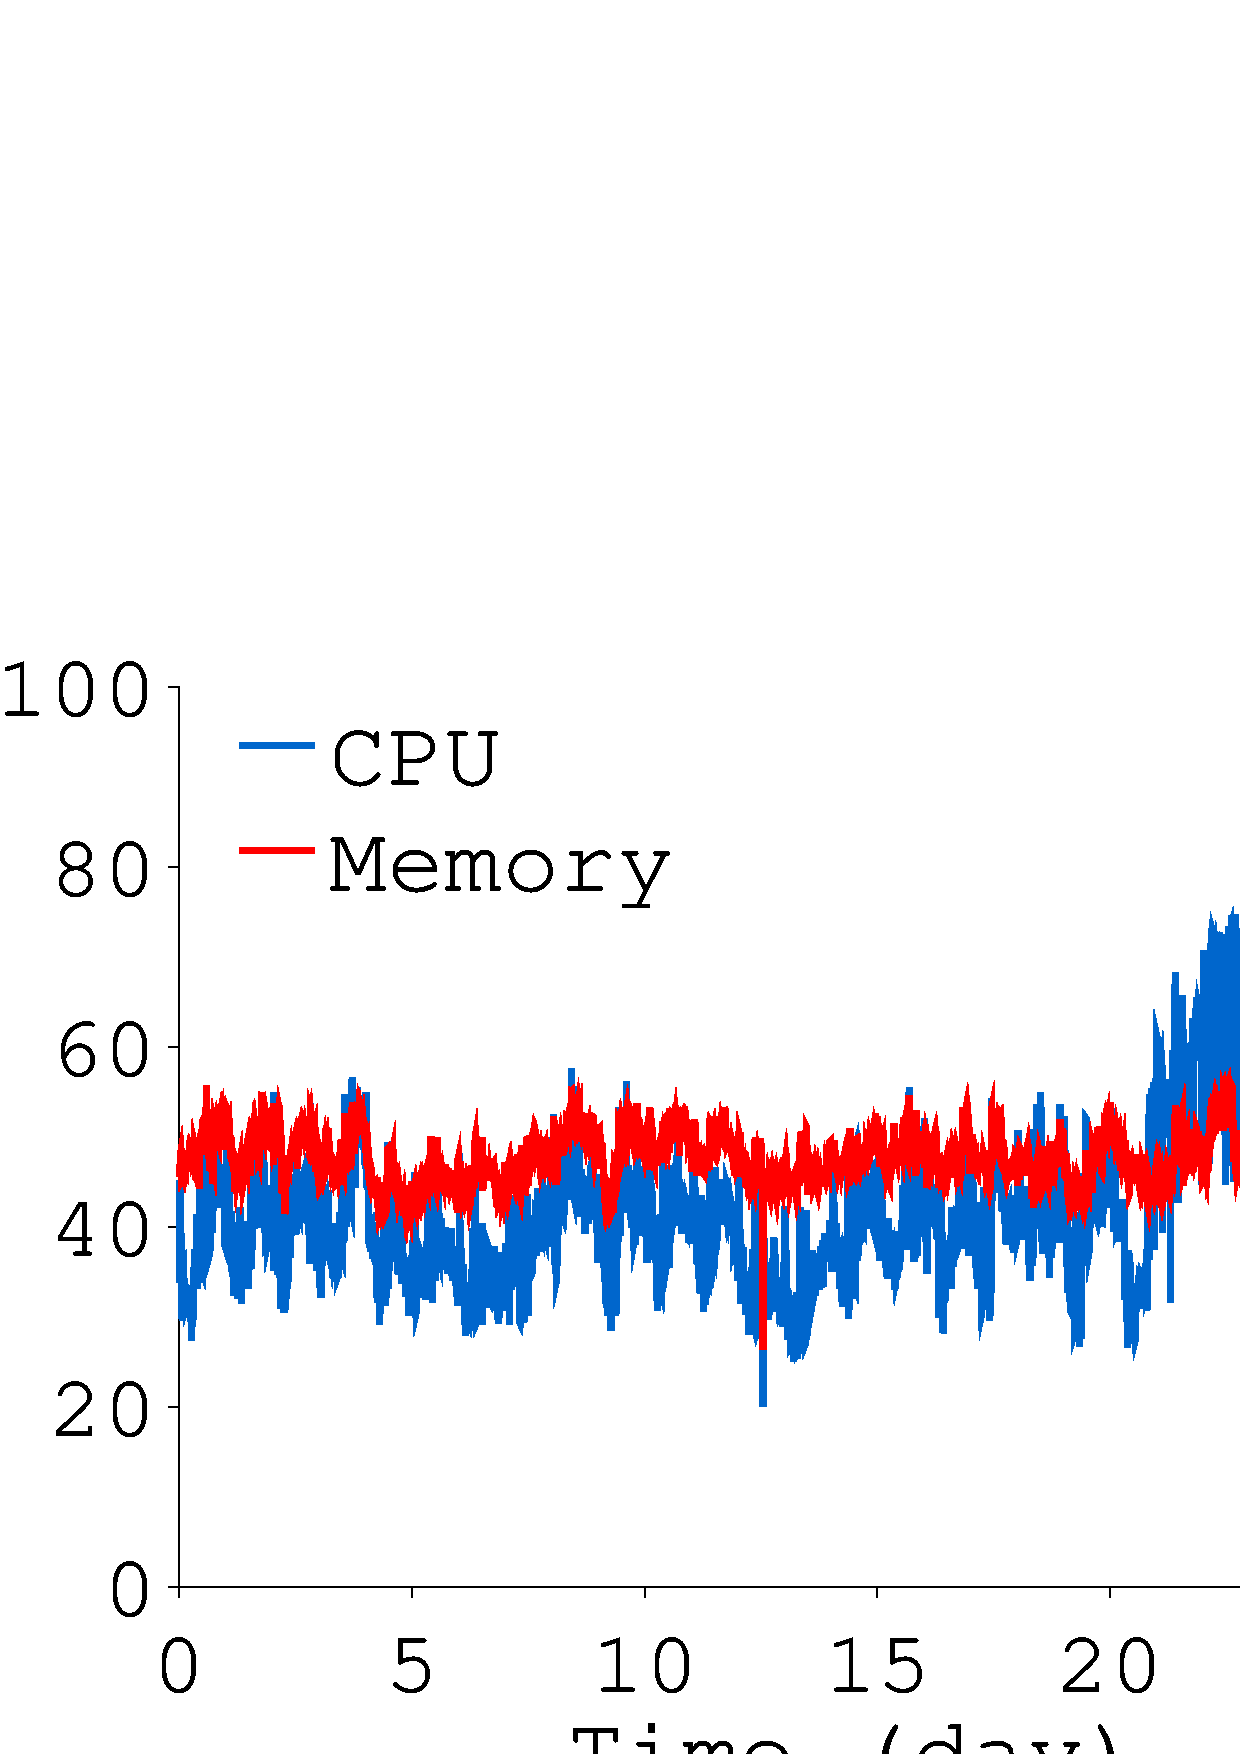
\includegraphics[width=3in]{lego/Figures/g_plot_google_util.pdf}}
    \caption[Google Cluster.]{Google Cluster.}
    \label{fig-googleutil}    
    \end{center}
\end{subfigure}
\begin{subfigure}{3in}
    \begin{center}    
    \centerline{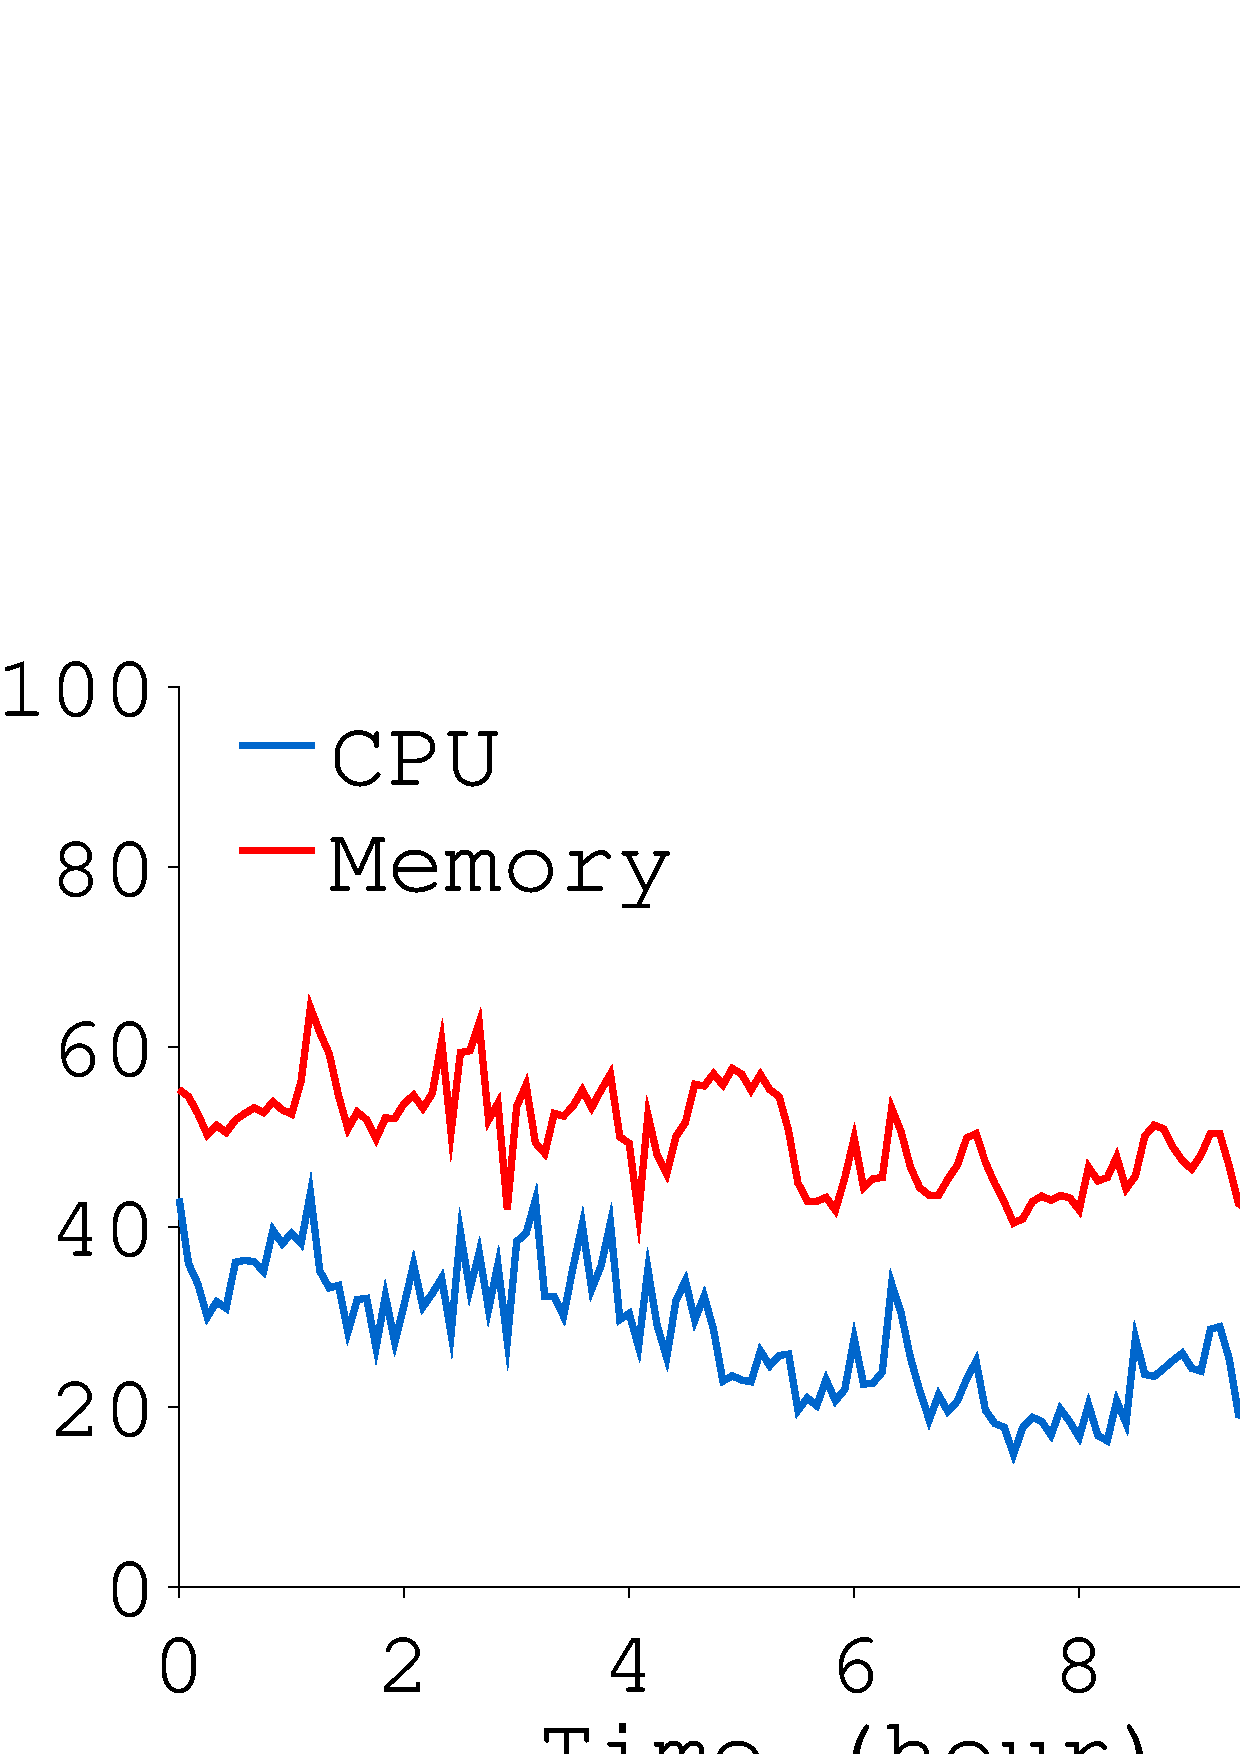
\includegraphics[width=3in]{lego/Figures/g_plot_ali_util.pdf}}    
    \caption[Alibaba Cluster.]{Alibaba Cluster.}
    \label{fig-aliutil}
    \end{center}    
\end{subfigure}
\caption[Data center resource utilization.]{Data center resource utilization.}
\label{fig-resource-anal}
\end{figure}
}
{
\begin{figure*}[t]
\begin{subfigure}{1.7in}
\begin{center}
\centerline{\includegraphics[width=1.7in]{lego/Figures/monolithic-arch.pdf}}
\caption[Monolithic OS.]{OSes Designed for Monolithic Servers.}
\label{fig-monolithic}
\end{center}
\end{subfigure}
\begin{minipage}{0.05in}
\hspace{0.05in}
\end{minipage}
\begin{subfigure}{1.8in}
\begin{center}
\centerline{\includegraphics[width=1.8in]{lego/Figures/multikernel-arch.pdf}}
\caption[Multikernel Architecture.]{Multi-kernel Architecture. \small{P-NIC: programmable NIC.}}
\label{fig-multikernel}
\end{center}
\end{subfigure}
\begin{minipage}{0.05in}
\hspace{0.05in}
\end{minipage}
\begin{subfigure}{2.5in}
\begin{center}
\centerline{\includegraphics[width=2.6in]{lego/Figures/lego-arch.pdf}}
\caption[Splitkernel Architecture.]{Splitkernel Architecture.}
\label{fig-splitkernel}
\end{center}
\end{subfigure}
\caption[Operating System Architecture.]{Operating System Architecture.}
\end{figure*}
}

This section
motivates the hardware resource disaggregation architecture
and discusses the challenges in managing disaggregated hardware.

\subsection{Limitations of Monolithic Servers}
\label{sec:lego:monolimit}
A monolithic server has been the unit of deployment and operation in datacenters for decades.
This long-standing {\em server-centric} architecture has several key limitations.

\noindent{\textit{\uline{Inefficient resource utilization.}}}
With a server being the physical boundary of resource allocation, 
it is difficult to fully utilize all resources in a datacenter~\cite{Barroso-COMPUTER,Quasar-ASPLOS,PowerNap}.
We analyzed two production cluster traces: a 29-day Google one~\cite{GoogleTrace}
and a 12-hour Alibaba one~\cite{AliTrace}.
Figure~\ref{fig-resource-anal} plots the aggregated CPU and memory utilization in the two clusters.
For both clusters, only around half of the CPU and memory are utilized.
Interestingly,
a significant amount of jobs are being evicted at the same time in these traces
(\eg, evicting low-priority jobs to make room for high-priority ones~\cite{Borg}).
One of the main reasons for resource under-utilization in these production clusters is 
the constraint that CPU and memory for a job have to be allocated from 
the same physical machine.

\noindent{\textit{\uline{Poor hardware elasticity.}}}
It is difficult to add, move, remove, or reconfigure hardware components
after they have been installed in a monolithic server~\cite{FB-Wedge100}. %, and
Because of this rigidity, datacenter owners have to plan out server configurations in advance.
However, with today's speed of change in application requirements, such plans have to be adjusted frequently,
and when changes happen, it often comes with waste in existing server hardware.

\noindent{\textit{\uline{Coarse failure domain.}}}
The failure unit of monolithic servers is coarse.
When a hardware component within a server fails, %(\eg, processor, memory chip, RAID controller), 
the whole server is often unusable and applications running on it can all crash.
Previous analysis~\cite{Failure-Disk-FAST07} found that motherboard, memory, CPU, power supply failures account for 
50\% to 82\% of hardware failures in a server.
Unfortunately, monolithic servers cannot continue to operate when any of these devices fail.

\noindent{\textit{\uline{Bad support for heterogeneity.}}}
Driven by application needs, new hardware technologies are finding their ways into modern datacenters~\cite{sigarch-dc}.
Datacenters no longer host only commodity servers with CPU, DRAM, and hard disks. 
They include non-traditional and specialized hardware like GPGPU~\cite{GPU-google,GPU-aws}, 
TPU~\cite{TPU}, 
DPU~\cite{DPU},
FPGA~\cite{Putnam14-FPGA,Amazon-F1}, %,SmartNIC-nsdi18},
non-volatile memory~\cite{Intel3DXpoint}, %,facebook-eurosys18},
and NVMe-based SSDs~\cite{everspin}.
The monolithic server model tightly couples hardware devices with each other and with a motherboard.
As a result, making new hardware devices work with existing servers is a painful and lengthy process~\cite{Putnam14-FPGA}.
%The current practice of making new hardware work is not only slow but also expensive.
Mover, datacenters often need to purchase new servers to host certain hardware.
Other parts of the new servers can go underutilized 
and old servers need to retire to make room for new ones.

\subsection{Hardware Resource Disaggregation}
The server-centric architecture is a bad fit for the fast-changing datacenter hardware, software, and cost needs.
There is an emerging interest in utilizing resources beyond a local machine~\cite{Gao16-OSDI},
such as distributed memory~\cite{Dragojevic14-FaRM,Nelson15-ATC,Aguilera17-SOCC,Novakovic16-SOCC} and network swapping~\cite{GU17-NSDI}. 
These solutions improve resource utilization over traditional systems.
However, they cannot solve all the issues of monolithic servers (\eg, the last three issues in \S\ref{sec:lego:monolimit}), 
since their hardware model is still a monolithic one.
To fully support the growing heterogeneity in hardware and to provide elasticity and flexibility at the hardware level, 
we should {\em break the monolithic server model.}% into flexible resource components.

We envision a {\em hardware resource disaggregation} architecture 
where hardware resources in traditional servers are disseminated into network-attached {\em hardware components}.
Each component has a controller and a network interface,
can operate on its own,
and is an {\em independent, failure-isolated} entity.

The disaggregated approach largely increases the flexibility of a datacenter.
Applications can freely use resources from any hardware component,
which makes resource allocation easy and efficient.
Different types of hardware resources can {\em scale independently}.
It is easy to add, remove, or reconfigure components.
New types of hardware components can easily be deployed in a datacenter ---
by simply enabling the hardware to talk to the network and adding a new network link to connect it.
Finally, hardware resource disaggregation enables fine-grain failure isolation, % because of decomposed hardware resources.
since one component failure will not affect the rest of a cluster.

Three hardware trends are making resource disaggregation feasible in datacenters.
First, network speed has grown by more than an order of magnitude and has become more scalable in the past decade % faster both in bandwidth and latency
with new technologies like Remote Direct Memory Access ({\it RDMA})~\cite{ibverbs} 
and new topologies and switches~\cite{FireBox-FASTKeynote,costa15-r2c2,Costa-WRSC14},
enabling fast accesses of hardware components that are disaggregated across the network.
InfiniBand will soon reach 200Gbps and sub-600 nanosecond speed~\cite{Mellanox-ConnectX6-IB},
being only 2\x\ to 4\x\ slower than main memory bus in bandwidth.
With main memory bus facing a bandwidth wall~\cite{BW-Wall-ISCA09},
future network bandwidth (at line rate) is even projected to exceed local DRAM bandwidth~\cite{CacheCloud-hotcloud18}.

Second, network interfaces are moving closer to hardware components,
with technologies like Intel OmniPath~\cite{OmniPath},
RDMA~\cite{ibverbs},
and NVMe over Fabrics~\cite{NVMe-fabrics-Inteltalk,NVMe-fabrics}.
As a result, hardware devices will be able to access network directly 
without the need to attach any processors. 

Finally, hardware devices are incorporating more processing power~\cite{Ahn15-PIM,Bojnordi12,Mellanox-SmartNIC,Mellanox-SmartNIC2,Agilio-SmartNIC,Junwhan-ISCA17},
allowing application and OS logics to be offloaded to hardware~\cite{Willow,Kaufmann16-ASPLOS}.
On-device processing power will enable system software to manage disaggregated hardware components locally.

With these hardware trends and the limitations of monolithic servers,
we believe that future datacenters will be able to largely benefit from hardware resource disaggregation.
In fact, there have already been several initial hardware proposals in resource disaggregation~\cite{OCP},
including disaggregated memory~\cite{Lim09-disaggregate,Scaleout-numa,Nitu18-EUROSYS}, 
disaggregated flash~\cite{FlashDisaggregation,ReFlex},
%new power state for disaggregated memory~\cite{Nitu18-EUROSYS},
Intel Rack-Scale System~\cite{IntelRackScale}, 
HP ``The Machine''~\cite{HP-TheMachine,HP-MemoryOS}, 
IBM Composable System~\cite{IBM-Composable},
and Berkeley Firebox~\cite{FireBox-FASTKeynote}.

\subsection{OSes for Resource Disaggregation}
Despite various benefits hardware resource disaggregation promises, 
it is still unclear how to manage or utilize disaggregated hardware in a datacenter.
Unfortunately, existing OSes and distributed systems cannot work well with this new architecture.
Single-node OSes like Linux view a server as the unit of management and assume all hardware components are local (Figure~\ref{fig-monolithic}).
A potential approach is to run these OSes on processors
and access memory, storage, and other hardware resources remotely.
Recent disaggregated systems like soNUMA~\cite{Scaleout-numa} take this approach.
However, this approach incurs high network latency and bandwidth consumption with remote device management,
misses the opportunity of exploiting device-local computation power,
and makes processors the single point of failure.

Multi-kernel solutions~\cite{Baumann-SOSP09,Barrelfish-DC,Helios-SOSP,fos-SOCC,Hive-SOSP} (Figure~\ref{fig-multikernel}) 
view different cores, processors, or programmable devices within a server separately 
by running a kernel on each core/device and using message passing to communicate across kernels.
These kernels still run in a single server and all access some common hardware resources in the server like memory and the network interface.
Moreover, they do not manage distributed resources or handle failures in a disaggregated cluster. 

There have been various distributed OS proposals,
most of which date decades back~\cite{Amoeba-Experience,Sprite,MOSIX}. %,V-System,Accent-SOSP,DEMOS-SOSP,Charlotte}.
Most of these distributed OSes manage a set of monolithic servers
instead of hardware components.

Hardware resource disaggregation is fundamentally different from the traditional monolithic server model.
A complete disaggregation of processor, memory, and storage 
means that when managing one of them, there will be no local accesses to the other two.
For example, processors will have no local memory or storage to store user or kernel data.
%Memory and storage components will only have limited processing power. %not have no local memory to serve as cache.
An OS also needs to manage distributed hardware resource and handle hardware component failure.
We summarize the following key challenges in building an OS for resource disaggregation,
some of which have previously been identified~\cite{HP-MemoryOS}.

\begin{itemize}
\item How to deliver good performance when application execution involves the access of network-partitioned disaggregated hardware
and current network is still slower than local buses?

\item How to locally manage individual hardware components with limited hardware resources?

%\item How to communicate across components?

\item How to manage distributed hardware resources?

\item How to handle a component failure without affecting other components or running applications?

\item What abstraction should be exposed to users and how to support existing datacenter applications?

\end{itemize}

Instead of retrofitting existing OSes to confront these challenges,
we take the approach of designing a new OS architecture from the ground up for hardware resource disaggregation.

\section{SuperNIC Overview}
\label{sec:overview}

%As discussed in \S\ref{sec:related}, although different existing network solutions provide some features of network disaggregation and consolidation, none of them meet all our target goals, thus necessitating the design of a new network solution.
This section gives a high-level overview of the overall architecture of the \snic\ platform and how to use it. %We defer the detailed description of \snic\ design to \S\ref{sec:design} and \S\ref{sec:dist}.

\bolditpara{Overall Architectures.}~~
We support two ways of attaching an \snic\ pool in a rack (Figure~\ref{fig-topology}).
In the first architecture, the \snic\ pool is an intermediate layer between endpoints (servers or devices) and the ToR switch.
Each \snic\ uses one port to connect to the ToR switch.
Optionally, all the \snic{}s can be directly connected to each other, \eg, with a ring topology.
All remaining ports in the \snic\ connect endpoints.
We expect each of these endpoint-connecting links to have high bandwidth (\eg, 100\Gbps) and the uplink to the switch to have the same or slightly higher bandwidth (\eg, 100\Gbps\ or 200\Gbps). 
%Differently, today's multi-host NICs break one link into several sub-links each with a fixed portion of the original link's bandwidth.\notearvind{This is the thing that the reviewer complained about.  Apparently, BF3 has a pcie switch at the ingress that removes this problem. We could skip making this point - but I think that reviewer is not on the SIGCOMM PC!}
%The sum of the link bandwidth at each endpoint that connects to an \snic\ can and should exceed the link bandwidth between the \snic\ and the ToR switch. 
%This is because different endpoints' loads peak at different times (\S\ref{sec:motivation-server}), and after \snic's consolidation, the aggregated traffic would mostly fit the \snic's uplink, as shown in Figure~\ref{fig-fb-alibaba}.
%
The second architecture attaches \snic{}s to the ToR switch, and endpoints directly attach to the ToR switch.
In this architecture, the ToR switch re-directs incoming or outgoing traffic to one or more \snic{}s. 
%and balances load when doing the redirection.
Note that for both architectures, the actual implementation could either package the network pool with the ToR switch to form a new ``switch box'' or be separated out as an pluggable pool. 


\if 0
\snic\ is a data-center-scale solution. %Any endpoint in a data center can be the sender and/or the receiver, and any 
An endpoint could either connect to an \snic\ or directly to a ToR switch.
A given \snic\ can connect different types of endpoints.
However, there is a potential benefit in connecting similar endpoints to an \snic.
Doing so offers more opportunity for resource consolidation, as similar endpoints (\eg, memory devices) are likely to use the same set of \nt{}s (\eg, encryption).
%On the other hand, the same type of endpoints are more likely to receive similar workloads (\eg, a replicated write sent to two memory devices) that could result in synchronized traffic peak and burden the \snic.

When an \snic\ fails, or its link to the ToR switch fails, if other links and the basic switching functionalities are still alive, the \snic\ would turn into a passthrough device, forwarding \nt{}s to other \snic{}s for processing.
When the entire \snic\ fails, the endpoints connected to it will be disconnected to the rest of the data center.
This failure could be viewed as equivalent to traditional ToR switch failure but with a smaller failure domain (only the endpoints under the failed \snic\ instead of the whole rack).
Data centers that desire stronger reliability~\cite{pangu-nsdi21} could use a multi-homed solution by connecting each endpoint to two \snic{}s.
\fi

\bolditpara{Requirements for endpoints and the last hop.}~~
For basic connectivity, an endpoint needs to have the equivalence of physical and link layers.
For reliable transmission, the link layer needs to provide basic reliability functionality if the reliable transport is offloaded to \snic.
This is because packets could still be corrupted or dropped during the point-to-point transmission between an endpoint and its connected \snic/switch (the last hop).
Thus, the endpoint's link layer should be able to detect corrupted or dropped packets. It will either correct the corruption or treat it as a lost packet and retransmit it.
%Since the connection is point-to-point, the reliable link layer only needs one logical flow and requires a small retransmission buffer.
%Our implementation uses only \fixme{XXX} more resource than an unreliable link layer.
%Since the connection is point-to-point, t
The link layer also requires a simple flow control to slow down packet sending when the \snic\ pool is overloaded or the application's fair share is exceeded.
%In addition, an endpoint should perform simple flow control of the last hop (\eg, by slowing down the transmission when receiving back pressure or using PFC).
%This addition is the only change to today's endpoints that use an unreliable link layer, and it is only needed when the reliable transport is offloaded to \snic.
%We choose 64\KB\ buffer size, which is more than sufficient in the worst case.
%Overall, our reliable link layer only uses 37\% more resources than an unreliable link layer.

%The above requirements are all that is needed for disaggregating network functionalities, and any endpoints that meets these requirements can work with \snic.
Any interconnect fabric that meets the above requirements can be used as the last-hop link.
PCIe is one such example, as it supports reliable data transfer and flow control.
%Our \snic\ prototype uses Ethernet and extends standard non-reliable link layer to handle the reliability and rely on Priority Flow Control (PFC) for flow control.
Our \snic\ prototype uses Ethernet as it is more flexible.
We use Priority Flow Control (PFC) for the one-hop flow control and add simple retransmission support.
%extend the unreliable Ethernet link layer with a small one-hop reliable retransmission.
%By design, \snic\ can work with different types of physical links between endpoints and the \snic. Our prototype uses regular Ethernet. Future extensions could use faster/tighter links like PCIe to further reduce latency overhead. 
Unlike a traditional reliable link layer, our {\em point-to-point} reliable link layer is lightweight, %(only 37\% more resources than an unreliable link layer with our implementation), 
as it only needs to maintain one logical flow and a small retransmission buffer for the small Bandwidth-Delay Product (BDP) of the last hop (64\KB\ in our prototype).

\if 0
%\fixme{TODO: Need to revisit the following three paragraphs depending on how much is implemented and evaluated. Also this is a place to shorten if we need more space.}
We envision three types of endpoints and different network features for them.
The first type is regular servers.
Servers could choose to offload a transport protocol, network functions, and/or application-specific tasks to \snic\ to save CPU cycles and/or to accelerate performance.
Since servers have plenty of memory (larger than or similar to what an \snic\ has), they are more fit to store data than \snic{}s.
One interesting architecture we explore is to offload a reliable transport to \snic\ but to have the server still buffer un-acknowledged packets until receiving an ACK from the receiver (which we refer to as an {\em end-to-end buffer}).
%In this case, \snic\ will discard packets after they leave the \snic, saving its memory for other tasks.

The second type is disaggregated devices that only serve as a request handler (\eg, a memory device that accepts memory alloc/read/write operations~\cite{clio-arxiv,ATC20-pDPM}). 
Such a device often has limited processing power and would offload most tasks such as a transport protocol, network functions like encryption, and device-specific functionalities like replication to \snic. 
Since it never serves as a request originator, there is no need to maintain any packet store, and a failure could be handled by having the client retry the entire request~\cite{clio-arxiv,homa-sigcomm18,1RMA-sigcomm20}.

The final type is disaggregated devices that could serve as request initiators (\eg, a disaggregated CPU or GPU device) but have little memory (because memory is disaggregated to memory devices~\cite{LegoOS}).
When offloading \nt{}s to \snic{}s, they do not have significant memory to maintain end-to-end buffers like regular servers.
On the other hand, if they do not buffer packets at all and rely on \snic\ to buffer un-acknowledged packets, errors can still happen when packets are not successfully delivered to the \snic. 
We propose a {\em one-hop buffer}---buffering a packet at the device only until the next hop (\ie, the \snic) acknowledges.
Doing so reduces the amount of time each packet is maintained and the overall memory consumption.
\fi

\bolditpara{Using SuperNIC.}~~
To use the \snic\ platform, users first write and deploy \nt{}s.
%The user can use any endpoints in the data center as the sender and the receiver (even if the endpoint is not connected to an \snic\ and connects directly to a ToR switch).
They specify which \snic\ (sender side or receiver side) to deploy an \nt.
Users also specify whether an \nt\ needs to access the packet payload and whether it needs to use on-board memory.
For the latter, we provide a virtual memory interface that gives each \nt\ its own virtual address space.
Optionally, users can specify which applications share the same \nt{}(s).
Currently, our FPGA prototype only supports \nt{}s written on FPGA (deployed as netlists).
Future implementation could extend \snic{}s to support p4 programs running on RMT pipelines~\cite{p4fpga-sosr17} and generic software programs running on a processor.

After all the \nt{}s that a user desires have been deployed, the user specifies one or multiple user-written or compiler-generated~\cite{clicknp-sigcomm16,NFP-sigcomm17} DAGs of the execution order of deployed \nt{}s. Users could also add more DAGs at run time. Compared to existing works which let users specify an NF DAG when deploying NFs~\cite{e2-sosp15,flowtags-nsdi14,clicknp-sigcomm16}, we allow more flexible usages and sharing of deployed \nt{}s. %Different from traditional NF execution flows that execute NFs in sequence, we allow multiple \nt{}s to execute in parallel. 
The \snic\ stores user-specified DAGs in its memory and assigns a unique identifier (UID) to each DAG.
At run time, each packet carries a UID, which \snic\ uses to fetch the DAG.




\if 0
For all the non-synchronization APIs, we offer two versions: synchronous and asynchronous.
While synchronous APIs are always strictly ordered within a user (and thus slower),
we relax the ordering of asynchronous APIs to a release consistency where operations can be executed out of order as long as 
1) read/write dependencies (WAR, RAW, WAW) are followed,
2) operations before a \fence\ must all complete before the \fence\ can return,
and 3) \fence{} operations are strictly ordered.
This release consistency is the same as architectures like ARMv8~\cite{ARMv8} and makes it possible for \sys\ to use a connectionless network layer with possible reordering (\S\ref{sec:network}).
Different users can share memory and can use \sys's synchronization primitives to achieve inter-user synchronization (\eg, using \tas\ to define critical section). 
\fi

\if 0
\sys\ is versatile in that there are many ways to use \sys's virtual memory view (we call it {\em \sys\ address space}).
Below and in Figure~\ref{fig-usage}, we list five typical ways to use \sys.
We implemented five applications with U2, U4, and U5;
U1 and U3 require building new hardware and/or OS/low-level systems, which are beyond this paper's scope.
%where client application processes can directly access disaggregated memory with their virtual memory addresses,
%no matter whether they run on \CN{}s or on \MN{}s.
%\sys\ only performs one address mapping: application virtual address to remote physical address (done at memory node),
%ordering

\stepcounter{case}
\boldpara{{\bf U\arabic{case}}: Entire virtual memory controlled by OS/hardware.}
A completely disaggregated solution like LegoOS~\cite{Shan18-OSDI}, where \CN{}s are compute devices with only CPU cache but no memory
can use \sys\ as the memory layer by sending \sys\ read/write requests to fulfill 
last-level-cache misses. % (called ExCache in LegoOS) misses.
With this usage, a \sys\ address space becomes the entire virtual memory address space
of a process, and \sys\ is completely transparent to application processes.

%usages
\stepcounter{case}
\boldpara{{\bf U\arabic{case}}: Extended virtual memory controlled by applications.}
%Applications run purely at \CN{}s and exploit \MN{}s for larger, dynamically allocated memory space.
%Note that the application ``virtual memory addresses'' \sys\ use (we call them \textit{\sys\ virtual memory address}es) 
%may not necessarily come from normal process memory address space.
%In fact, there are three ways to use \sys, and they have their own interpretation of what \sys\ virtual memory addresses mean,
%as illustrated in Figure~\ref{fig-arch}.
Without changing existing server hardware or OS at \CN{}s, 
an application process can explicitly call \sys\ APIs by linking \syslib\ which creates an extra \textit{remote virtual memory address space} (\ie, a \sys\ address space)
that is separate from the process' normal (local) virtual memory address space.
Applications have precise control over what and when to use disaggregated memory and can use or implement high-level APIs like pointer chasing.

%The returned addresses of \alloc\ and input addresses of \sysread/\syswrite requests will all be virtual addresses in this space ({\em dvma-vaddr}).

\stepcounter{case}
\boldpara{{\bf U\arabic{case}}: Remote memory space controlled by a middle layer.}
A system layer like a remote-memory swap system~\cite{InfiniSwap,FastSwap} or a language runtime~\cite{Semeru}
can sit on top of \sys\ and use a \sys\ address space as its own managed space (\eg, a swap partition, a JVM heap).
Applications on top of such a layer can transparently access larger memory backed by \sys.
%Second, applications can sit on top a remote-memory swap system like FastSwap~\cite{FastSwap} and InfiniSwap~\cite{InfiniSwap},
%which uses \sys\ virtual memory addresses as swap partition address ({\em swap-vaddr}) and performs \sys\ read/write to swap in/out disaggregated memory.

%Using client process virtual memory addresses also has the benefit that disaggregated memory can potentially be 
%integrated into client machine's memory micro-architecture~\cite{Lim09-disaggregate}.

\stepcounter{case}
\boldpara{{\bf U\arabic{case}}: Memory services running at \MN{}s.}
Users can deploy {\em memory services} that run entirely at \MN{}s (\eg, 
an in-memory key-value store or object data store) 
and expose their own interface (\eg, key-value get/set) 
to the clients of these services that run at \CN{}s.
These services can be deployed to \sysboard's programmable hardware and/or software platforms.
Each memory service has its own isolated \sys\ address space and can use \sys's APIs, 
which makes hardware implementation easier and execution safer.

\stepcounter{case}
\boldpara{{\bf U\arabic{case}}: Partial computation offloading.}
While U1, U2, and U3 perform computation completely at \CN{}s and U4 performs computation entirely at \MN{}s,
applications can also split their computation across \CN{} and \MN{}.
%An application can offload some of its computation tasks to an \MN{} (run in hardware or software).
\sys\ offers a {\em unified} address space for an application's \CN{} and \MN{} parts.
These parts are treated as different \sys\ threads. 
As explained earlier, if they cache shared data locally, they need to have their own mechanism to make the cache coherent, if desired.
\sys\ offers synchronization primitives to assist them work with their shared data.
%with each being treated as a traditional thread (\eg, \CN{} and \MN{} threads can be synchronized using \tas\ and other \sys\ synchronization primitives).
%\stepcounter{principle}
%\ulinebfpara{Principle \arabic{principle}:}
%\textit{The disaggregated memory abstraction should face client processes}.

\fi

\section{\lego\ Design}
\label{sec:lego:design}

Based on the \splitkernel\ architecture,
we built {\em \lego}, the first OS designed for hardware resource disaggregation.
\lego\ is a research prototype that demonstrates the feasibility of the \splitkernel\ design,
but it is not the only way to build a \splitkernel.
\lego' design targets three types of hardware components:
processor, memory, and storage,
and we call them {\em \pcomponent, \mcomponent}, and {\em \scomponent}.

This section first introduces the abstraction \lego\ exposes to users
and then describes the hardware architecture of components \lego\ runs on.
Next, we explain the design of \lego' process, memory, and storage \microos{}s.
Finally, we discuss \lego' global resource management and failure handling mechanisms.

Overall, \lego\ achieves the following design goals:

\begin{itemize}

\item Clean separation of process, memory, and storage functionalities.

\item Monitors run at hardware components and fit device constraints.

\item Comparable performance to monolithic Linux servers.

\item Efficient resource management and memory failure handling, both in space and in performance. % and performance-efficient memory replication scheme.

\item Easy-to-use, backward compatible user interface.

\item Supports common Linux system call interfaces.

\end{itemize}

\subsection{Abstraction and Usage Model}
\lego\ exposes a distributed set of {\em virtual nodes}, or {\em \vnode}, to users.
From users' point of view, a \vnode\ is like a virtual machine. 
Multiple users can run in a \vnode\ and each user can run multiple processes.
Each \vnode\ has a unique ID, a unique virtual IP address, %({\em \vip}),
and its own storage mount point. % ({\em \vmount}).
\lego\ protects and isolates the resources given to each \vnode\ from others.
Internally, one \vnode\ can run on multiple \pcomponent{}s, multiple \mcomponent{}s,
and multiple \scomponent{}s.
At the same time, each hardware component can host resources for more than one \vnode.
The internal execution status is transparent to \lego\ users;
they do not know which physical components their applications run on.

With \splitkernel's design principle of components not being coherent,
\lego\ does not support writable shared memory across processors. %execute application threads that need to have shared write access to common memory.
\lego\ assumes that threads within the same process access shared memory
and threads belonging to different processes do not share writable memory,
and \lego\ makes scheduling decision based on this assumption (\S\ref{sec:lego:proc-scheduling}).
Applications that use shared writable memory across processes (\eg, with MAP\_SHARED)
will need to be adapted to use message passing across processes.
We made this decision because writable shared memory across processes is rare 
(we have not seen a single instance in the datacenter applications we studied),
and supporting it makes both hardware and software more complex 
(in fact, we have implemented this support but later decided not to include it because of its complexity).

One of the initial decisions we made when building \lego\ is to support the Linux system call interface 
and unmodified Linux ABI,
because doing so can greatly ease the adoption of \lego.
Distributed applications that run on Linux can seamlessly run on a \lego\ cluster
by running on a set of \vnode{}s. % and using their virtual IP addresses to communicate.

\subsection{Hardware Architecture}
\label{sec:lego:hardware}
{
\begin{figure}[th]
\begin{center}
\centerline{\includegraphics[width=0.8\textwidth]{lego/Figures/hwarch.pdf}}
\caption[\lego\ \pcomponent\ and \mcomponent\ Architecture.]{\lego\ \pcomponent\ and \mcomponent\ Architecture.}
\label{fig-lego-hw-arch}
\end{center}
\end{figure}
}

\lego\ \pcomponent, \mcomponent, and \scomponent\ are independent devices,
each having their own hardware controller and network interface (for \pcomponent, the hardware controller is the processor itself).
Our current hardware model uses CPU in \pcomponent, 
DRAM in \mcomponent, and SSD or HDD in \scomponent.
We leave exploring other hardware devices for future work.

To demonstrate the feasibility of hardware resource disaggregation,
we propose a \pcomponent{} and an \mcomponent\ architecture designed 
within today's network, processor, and memory performance and hardware constraints
(Figure~\ref{fig-lego-hw-arch}).

\noindent{\textit{\uline{Separating process and memory functionalities.}}}
\lego\ moves all hardware memory functionalities to \mcomponent{}s 
(e.g., page tables, TLBs) and leaves {\em only} caches at the \pcomponent{} side. 
With a clean separation of process and memory hardware units, 
the allocation and management of memory can be completely transparent to \pcomponent{}s.
Each \mcomponent{} can choose its own memory allocation technique
and virtual to physical memory address mappings (\eg, segmentation). 

\noindent{\textit{\uline{Processor virtual caches.}}}
After moving all memory functionalities to \mcomponent{}s,  
\pcomponent{}s will only see virtual addresses and have to use virtual memory addresses to access its caches. 
Because of this, \lego\ organizes all levels of \pcomponent{} caches as {\em virtual caches}~\cite{Goodman-ASPLOS87,Wang-ISCA89},
\ie, virtually-indexed and virtually-tagged caches.

A virtual cache has two potential problems, commonly known as synonyms and homonyms~\cite{CacheMemory82}.
Synonyms happens when a physical address maps to multiple virtual addresses (and thus multiple virtual cache lines) 
as a result of memory sharing across processes,
and the update of one virtual cache line will not reflect to other lines that share the data.
Since \lego\ does not allow writable inter-process memory sharing,
it will not have the synonym problem.
The homonym problem happens when two address spaces use the same virtual address for their own different data.
Similar to previous solutions~\cite{OVC}, we solve homonyms by storing an address space ID (ASID) with each cache line,
and differentiate a virtual address in different address spaces using ASIDs.

\noindent{\textit{\uline{Separating memory for performance and for capacity.}}}
Previous studies~\cite{Gao16-OSDI,GU17-NSDI} and our own show that today's network speed 
cannot meet application performance requirements if all memory accesses are across the network. 
Fortunately, many modern datacenter applications exhibit strong memory access temporal locality.
For example, we found 90\% of memory accesses in PowerGraph~\cite{Gonzalez12-OSDI} go to just 0.06\% of total memory
and 95\% go to 3.1\% of memory
(22\% and 36\% for TensorFlow~\cite{TensorFlow} respectively,
5.1\% and 6.6\% for Phoenix~\cite{Ranger07-HPCA}).
%PG 90% 0.0063G 95% 0.301G 100% 9.68G
%TF 90% 0.608G 95% 0.968G 100% 2.7G

With good memory-access locality, we propose to %separate hardware memory into two categories and organize them differently:
leave a small amount of memory (\eg, 4\GB) at each \pcomponent{}
and move most memory across the network (\eg, few TBs per \mcomponent{}).
\pcomponent{}s' local memory can be regular DRAM 
or the on-die HBM~\cite{HBM-JEDEC,Knights-Landing},
and \mcomponent{}s use DRAM or NVM.

Different from previous proposals~\cite{Lim09-disaggregate}, 
we propose to organize \pcomponent{}s' DRAM/HBM as cache rather than main memory
for a clean separation of process and memory functionalities.
We place this cache under the current processor Last-Level Cache (LLC)
and call it an extended cache, or {\em \excache}.
\excache\ serves as another layer in the memory hierarchy between LLC and memory across the network.
With this design, \excache\ can serve hot memory accesses fast, while \mcomponent{}s can provide the capacity applications desire. 

\excache\ is a virtual, inclusive cache,
and we use a combination of hardware and software to manage \excache.
Each \excache\ line has a (virtual-address) tag and two access permission bits (one for read/write and one for valid).
These bits are set by software when a line is inserted to \excache\ and checked by hardware at access time.
For best hit performance, the hit path of \excache\ is handled purely by hardware
--- the hardware cache controller maps a virtual address to an \excache\ set, 
fetches and compares tags in the set, and on a hit, fetches the hit \excache\ line.
Handling misses of \excache\ is more complex than with traditional CPU caches, 
and thus we use \lego\ to handle the miss path of \excache\ (see \S\ref{sec:lego:excachemgmt}).

Finally, we use a small amount of DRAM/HBM at \pcomponent{} for \lego' own kernel data usages,
accessed directly with physical memory addresses and managed by \lego. 
\lego\ ensures that all its own data fits in this space to avoid going to \mcomponent{}s.

With our design, \pcomponent{}s do not need any address mappings:
\lego\ accesses all \pcomponent{}-side DRAM/HBM using physical memory addresses
and does simple calculations to locate the \excache\ set for a memory access.
Another benefit of not handling address mapping at \pcomponent{}s and moving TLBs to \mcomponent{}s 
is that \pcomponent{}s do not need to access TLB or suffer from TLB misses,
potentially making \pcomponent{} cache accesses faster~\cite{Kaxiras-ISCA13}.
%We use software~\cite{softvm-HPCA97,Tsai-ISCA17} (\lego) to manage \excache\ and the kernel physical memory,
%although they can all be implemented in hardware too.

\subsection{Process Management}
The \lego\ {\em process \microos{}} runs in the kernel space of a \pcomponent\
and manages the \pcomponent's CPU cores and \excache. 
\pcomponent{}s run user programs in the user space.

\subsubsection{Process Management and Scheduling}
\label{sec:lego:proc-scheduling}
At every \pcomponent, \lego\ uses a simple local thread scheduling model 
that targets datacenter applications 
(we will discuss global scheduling in \S~\ref{sec:lego:grm}).
\lego\ dedicates a small amount of cores for kernel background threads 
(currently two to four)
and uses the rest of the cores for application threads.
When a new process starts, \lego\ uses a global policy to choose a \pcomponent{} for it (\S~\ref{sec:lego:grm}).
Afterwards, \lego\ schedules new threads the process spawns on the same \pcomponent{} 
by choosing the cores that host fewest threads.
After assigning a thread to a core, 
we let it run to the end with no scheduling or kernel preemption under common scenarios.
For example, we do not use any network interrupts 
and let threads busy wait on the completion of outstanding network requests, 
since a network request in \lego\ is fast 
(\eg, fetching an \excache\ line from an \mcomponent\ takes around 6.5\mus).
\lego\ improves the overall processor utilization in a disaggregated cluster,
since it can freely schedule processes on any \pcomponent{}s without considering memory allocation.
Thus, we do not push for perfect core utilization when scheduling individual threads
and instead aim to minimize scheduling and context switch performance overheads.
Only when a \pcomponent{} has to schedule 
more threads than its cores will
\lego\ start preempting threads on a core.

\subsubsection{\excache\ Management}
\label{sec:lego:excachemgmt}
\lego\ process \microos\ configures and manages \excache.
During the \pcomponent{}'s boot time, \lego\ configures the set associativity of \excache\
and its cache replacement policy.
While \excache\ hit is handled completely in hardware, 
\lego\ handles misses in software.
When an \excache\ miss happens, 
the process \microos\ fetches the corresponding line from an \mcomponent\ and inserts it to \excache.
If the \excache\ set is full, the process \microos\ first evicts a line in the set.
It throws away the evicted line if it is clean
and writes it back to an \mcomponent{} if it is dirty.
\lego\ currently supports two eviction policies: FIFO and LRU.
For each \excache\ set, \lego\ maintains a FIFO queue (or an approximate LRU list)
and chooses \excache\ lines to evict based on the corresponding policy (see \S\ref{sec:lego:procimpl} for details).

\subsubsection{Supporting Linux Syscall Interface}
One of our early decisions is to support Linux ABIs for backward compatibility
and easy adoption of \lego.
A challenge in supporting the Linux system call interface is that 
many Linux syscalls are associated with {\em states},
information about different Linux subsystems that is stored with each process 
and can be accessed by user programs across syscalls.
For example, Linux records the states of a running process' open files, socket connections, and several other entities,
and it associates these states with file descriptors ({\em fd}s) that are exposed to users.
In contrast, \lego\ aims at the clean separation of OS functionalities.
With \lego' stateless design principle, each component only stores information about its own resource
and each request across components contains all the information that the destination component needs to handle the request.
To solve this discrepancy between the Linux syscall interface and \lego' design, 
we add a layer on top of \lego' core process \microos\ at each \pcomponent\ to store Linux states
and translate these states and the Linux syscall interface to \lego' internal interface.

\subsection{Memory Management}

We use \mcomponent{}s for three types of data:
anonymous memory (\ie, heaps, stacks), 
memory-mapped files, and storage buffer caches.
The \lego\ {\em memory \microos{}}
manages both the virtual and physical memory address spaces,
their allocation, deallocation, and memory address mappings.
It also performs the actual memory read and write.
No user processes run on \mcomponent{}s 
and they run completely in the kernel mode
(same is true for \scomponent{}s). 

\lego\ lets a process address space span multiple \mcomponent{}s
to achieve efficient memory space utilization and high parallelism.
Each application process uses one or more \mcomponent{}s to host its data
and a {\em home \mcomponent},
an \mcomponent\ that initially loads the process, 
accepts and oversees all system calls related to virtual memory space management
(\eg, \brk, \mmap, \munmap, and \mremap).
\lego\ uses a global memory resource manager ({\em \gmm}) to assign a home \mcomponent{} to each new process at its creation time.
A home \mcomponent\ can also host process data.

\subsubsection{Memory Space Management}
\noindent{\textit{\uline{Virtual memory space management.}}}
We propose a two-level approach to manage distributed virtual memory spaces,
where the home \mcomponent\ of a process makes coarse-grained, high-level virtual memory allocation decisions
and other \mcomponent{}s perform fine-grained virtual memory allocation.
This approach minimizes network communication during both normal memory accesses and virtual memory operations,
while ensuring good load balancing and memory utilization.
Figure~\ref{fig-dist-vma} demonstrates the data structures used. % in virtual memory space management.

At the higher level, we split each virtual memory address space into coarse-grained, fix-sized {\em virtual regions},
or {\em \vregion{}s} (\eg, of 1\GB).
Each \vregion\ that contains allocated virtual memory addresses (an active \vregion) is {\em owned} by an \mcomponent{}.
The owner of a \vregion\ handles all memory accesses and virtual memory requests within the \vregion.

{
\begin{figure}[th]
\begin{minipage}{\figWidth}
\begin{center}
\centerline{\includegraphics[width=2.8in]{Figures/dist-vma.pdf}}
%\vspace{-0.1in}
\mycaption{fig-dist-vma}{Distributed Memory Management.}
{
}
\end{center}
\end{minipage}
\vspace{-0.15in}
\end{figure}
}

The lower level stores user process virtual memory area ({\em vma}) information,
such as virtual address ranges and permissions, in {\em vma trees}.
The owner of an active \vregion\ stores a vma tree for the \vregion,
with each node in the tree being one vma.
A user-perceived virtual memory range can split across multiple \mcomponent{}s,
but only one \mcomponent{} owns a \vregion.

\vregion\ owners perform the actual virtual memory allocation and vma tree set up.
A home \mcomponent{} can also be the owner of \vregion{}s,
but the home \mcomponent{} does not maintain any information about memory that belongs to \vregion{}s owned by other \mcomponent{}s.
It only keeps the information of which \mcomponent{} owns a \vregion\ (in a {\em \vregion\ array})
and how much free virtual memory space is left in each \vregion.
These metadata can be easily reconstructed if a home \mcomponent{} fails.

When an application process wants to allocate a virtual memory space,
the \pcomponent{} forwards the allocation request 
to its home \mcomponent{} (\circled{1} in Figure~\ref{fig-dist-vma}).
The home \mcomponent{} uses its stored information of available virtual memory space in \vregion{}s
to find one or more \vregion{}s that best fit the requested amount of virtual memory space.
If no active \vregion\ can fit the allocation request, the home \mcomponent{} makes a new \vregion\ active and 
contacts the \gmm\ (\circled{2} and \circled{3}) to find a candidate \mcomponent{} to own the new \vregion.
\gmm\ makes this decision based on available physical memory space and access load on different \mcomponent{}s (\S~\ref{sec:lego:grm}).
If the candidate \mcomponent\ is not the home \mcomponent{}, the home \mcomponent{} next forwards the request to that \mcomponent\ (\circled{4}),
which then performs local virtual memory area allocation and sets up the proper vma tree. 
Afterwards, the \pcomponent{} directly sends memory access requests to the owner of the \vregion\ where the memory access falls into
(\eg, \circled{a} and \circled{c} in Figure~\ref{fig-dist-vma}).


\lego' mechanism of distributed virtual memory management is efficient and it cleanly separates memory operations from \pcomponent{}s.
\pcomponent{}s hand over all memory-related system call requests to \mcomponent{}s
and only cache a copy of the \vregion\ array for fast memory accesses.
To fill a cache miss or to flush a dirty cache line, 
a \pcomponent{} looks up the cached \vregion\ array to find its owner \mcomponent{} and sends the request to it.

\noindent{\textit{\uline{Physical memory space management.}}}
Each \mcomponent\ manages the physical memory allocation for data that falls into the
\vregion\ that it owns.
Each \mcomponent{} can choose their own way of physical memory allocation
and own mechanism of virtual-to-physical memory address mapping.


\subsubsection{Optimization on Memory Accesses}
\label{sec:lego:zerofill}
With our strawman memory management design, 
all \excache\ misses will go to \mcomponent{}s.
We soon found that a large performance overhead in running real applications 
is caused by filling empty \excache, \ie, {\em cold misses}.
To reduce the performance overhead of cold misses, we propose a technique 
to avoid accessing \mcomponent\ on first memory accesses.

The basic idea is simple: since the initial content of anonymous memory 
(non-file-backed memory) is zero, %undefined and can be any data, 
\lego\ can directly allocate a cache line with empty content
in \excache\ for the first access to 
anonymous memory instead of going to \mcomponent\
(we call such cache lines {\em p-local lines}).
When an application creates a new anonymous memory region, the process \microos\ records its address range and permission.
The application's first access to this region will be an \excache\ miss and it will trap to \lego.
\lego\ process \microos\ then allocates an \excache\ line, fills it with zeros, 
and sets its R/W bit according to the recorded memory region's permission.
Before this p-local line is evicted, it only lives in the \excache.
No \mcomponent{}s are aware of it or will allocate physical memory or a virtual-to-physical memory mapping for it.
When a p-local cache line becomes dirty and needs to be flushed, 
the process \microos\ sends it to its owner \mcomponent, which then
allocates physical memory space and establishes a virtual-to-physical memory mapping.
Essentially, \lego\ {\em delays physical memory allocation until write time}.
Notice that it is safe to only maintain p-local lines at a \pcomponent{} \excache\ 
without any other \pcomponent{}s knowing them, 
since \pcomponent{}s in \lego\ do not share any memory
and other \pcomponent{}s will not access this data.

\subsection{Storage Management}
\lego\ supports a hierarchical file interface that is backward compatible with POSIX 
through its \vnode\ abstraction. 
Users can store their directories and files under their \vnode{}s' mount points
and perform normal read, write, and other accesses to them.

\lego\ implements core storage functionalities at \scomponent{}s.
To cleanly separate storage functionalities, \lego\ uses a stateless storage server design, 
where each I/O request to the storage server contains all the information needed to 
fulfill this request, \eg, full path name, absolute file offset,
similar to the server design in NFS v2~\cite{Sandberg-NFS-85}.

While \lego\ supports a hierarchical file use interface,
internally, \lego\ storage \microos\ treats (full) directory and file paths just as unique names of a file
and place all files of a \vnode\ under one internal directory at the \scomponent{}.
To locate a file, \lego\ storage \microos\ maintains a simple hash table with the full paths of files (and directories) as keys.
From our observation, most datacenter applications only have a few hundred files or less.
Thus, a simple hash table for a whole \vnode\ is sufficient to achieve good lookup performance.
Using a non-hierarchical file system implementation largely reduces the complexity of \lego' file system,
making it possible for a storage \microos\ to fit in storage devices controllers that have limited processing power~\cite{Willow}.

\lego\ places the storage buffer cache at \mcomponent{}s
rather than at \scomponent{}s, because \scomponent{}s can only host a limited amount of internal memory.
\lego\ memory \microos\ manages the storage buffer cache by simply performing insertion, lookup, and deletion of buffer cache entries.
For simplicity and to avoid coherence traffic, we currently place the buffer cache of one file
under one \mcomponent{}.
When receiving a file read system call, the \lego\ process \microos\ first uses its extended Linux state layer to 
look up the full path name, then passes it with the requested offset and size to the \mcomponent\ that holds the file's buffer cache.
This \mcomponent\ will look up the buffer cache and returns the data to \pcomponent\ on a hit.
On a miss, \mcomponent\ will forward the request to the \scomponent\ that stores the file, 
which will fetch the data from storage device and return it to the \mcomponent.
The \mcomponent\ will then insert it into the buffer cache and returns it to the \pcomponent.
Write and fsync requests work in a similar fashion.

\subsection{Global Resource Management}
\label{sec:lego:grm}
\lego\ uses a two-level resource management mechanism.
At the higher level, \lego\ uses three global resource managers for process, memory, and storage resources, 
{\em \gpm, \gmm}, and {\em \gsm}.
These global managers perform coarse-grained global resource allocation and load balancing,
and they can run on one normal Linux machine.
Global managers only maintain approximate resource usage and load information.
They update their information either when they make allocation decisions 
or by periodically asking \microos{}s in the cluster.
At the lower level, each \microos\ can employ its own policies and mechanisms to manage its local resources.

For example, process \microos{}s allocate new threads locally 
and only ask \gpm\ when they need to create a new process.
\gpm\ chooses the \pcomponent{} that has the least amount of threads based on its maintained approximate information.
Memory \microos{}s allocate virtual and physical memory space on their own.
Only home \mcomponent{} asks \gmm\ when it needs to allocate a new \vregion.
\gmm\ maintains approximate physical memory space usages and memory access load by periodically asking \mcomponent{}s
and chooses the memory with least load among all the ones that have at least \vregion\ size of free physical memory.

\lego\ decouples the allocation of different resources and 
can freely allocate each type of resource from a pool of components.
Doing so largely improves resource packing compared to a monolithic server cluster
that packs all type of resources a job requires within one physical machine.
Also note that \lego\ allocates hardware resources only {\em on demand}, 
\ie, when applications actually create threads or access physical memory.
This on-demand allocation strategy further improves \lego' resource packing efficiency
and allows more aggressive over-subscription in a cluster.

\subsection{Reliability and Failure Handling}
\label{sec:lego:failure}
After disaggregation, \pcomponent{}s, \mcomponent{}s, and \scomponent{}s can all fail independently.
Our goal is to build a reliable disaggregated cluster that has the same or lower application failure rate
than a monolithic cluster.
As a first (and important) step towards achieving this goal, %building a reliable disaggregated cluster,
we focus on providing memory reliability by handling \mcomponent\ failure in the current version of \lego\ because of three observations.
First, when distributing an application's memory to multiple \mcomponent{}s, 
the probability of memory failure increases and not handling \mcomponent\ failure will cause applications to fail more often 
on a disaggregated cluster than on monolithic servers.
Second, since most modern datacenter applications
already provide reliability to their distributed storage data %(usually through some form of redundancy)
and the current version of \lego\ does not split a file across \scomponent,
we leave providing storage reliability to applications.
Finally, since \lego\ does not split a process across \pcomponent{}s,
the chance of a running application process being affected by the failure of a \pcomponent\ is similar to 
one affected by the failure of a processor in a monolithic server.
Thus, we currently do not deal with \pcomponent\ failure and leave it for future work.

A naive approach to handle memory failure is to perform a full replication of memory content over two or more \mcomponent{}s.
This method would require at least 2\x\ memory space,
making the monetary and energy cost of providing reliability prohibitively high (the same reason why RAMCloud~\cite{Ongaro11-RamCloud} does not replicate in memory).
Instead, we propose a space- and performance-efficient approach to provide in-memory data reliability in a best-effort way.
Further, since losing in-memory data will not affect user persistent data,
we propose to provide memory reliability in a best-effort manner.

We use one primary \mcomponent, one secondary \mcomponent, and a backup file in \scomponent\ for each vma.
A \mcomponent{} can serve as the primary for some vma and the secondary for others.
The primary stores all memory data and metadata.
\lego\ maintains a small append-only log at the secondary \mcomponent{}
and also replicates the vma tree there.
When \pcomponent{} flushes a dirty \excache\ line, 
\lego\ sends the data to both primary and secondary in parallel (step \circled{a} and \circled{b} in Figure~\ref{fig-dist-vma})
and waits for both to reply (\circled{c} and \circled{d}).
In the background, the secondary \mcomponent\ flushes the backup log to a \scomponent{},
which writes it to an append-only file.

If the flushing of a backup log to \scomponent\ is slow and the log is full, 
we will skip replicating application memory.
If the primary fails during this time, \lego\ simply reports an error to application.
Otherwise when a primary \mcomponent\ fails, we can recover memory content 
by replaying the backup logs on \scomponent\ and in the secondary \mcomponent.
When a secondary \mcomponent\ fails, we do not reconstruct anything 
and start replicating to a new backup log on another \mcomponent{}.


\section{\sys\ Implementation}
\label{sec:impl}

Apart from challenges discussed in \S\ref{sec:design}, our implementation of \sys\ also needs to overcome several practical challenges, for example, how can different hardware components most efficiently work together in \sysboard, how to minimize software overhead in \syslib. 
This section describes how we implemented \sysboard\ and \syslib, focusing on the new techniques we designed to overcome these challenges.
Currently, \sys\ consists of 24.6K SLOC (excluding computation offloads and third-party IPs).
They include 5.6K SLOC in SpinalHDL~\cite{SpinalHDL} and 2K in C HLS for FPGA hardware, and 17K in C for \syslib\ and ARM software.
We use vendor-supplied interconnect and DDR IPs, and an open-source MAC and PHY network stack~\cite{Corundum-FCCM20}.

\ulinebfpara{\sysboard\ Prototyping.}~~
%\label{sec:impl}
\if 0
By design (Figure~\ref{fig-coremem}), a \sysboard\ consists of an data path ASIC, a small FPGA, and a few low-power cores,
a network interface (at least one port of 100\Gbps\ or higher), and an array of off-chip DRAMs of at least hundreds of GBs.
All components except the DRAMs are expected to be integrated into a single chip.
The ASIC is dedicated to fixed logics including \sys's virtual memory fast path and network system (L1+L2 MAC).
The software cores run the virtual memory and offloads' slow paths.
The FPGA runs offloads' fast paths.
\fi
We prototyped \sysboard\ with a low-cost (\$2495 retail price) Xilinx MPSoC board~\cite{ZCU106} and build the hardware fast path (which is anticipated to be built in ASIC) with FPGA.
All \sys's FPGA modules run at 250\,MHz clock frequency and 512-bit data width.
They all %(network, pre-processor, core memory) are able to 
achieve an {\em Initiation Interval} ({\em II}) of one
(II is the number of clock cycles between the start time
of consecutive loop iterations, and it decides the maximum
achievable bandwidth). Achieving II of one is not easy and
requires careful pipeline design in all the modules. With II one, our data path can
achieve a maximum of 128\Gbps\ throughput even with just the slower FPGA clock frequency and would be higher with real ASIC implementation.

Our prototyping board consists of a small FPGA with 504K logic cells (LUTs) and 4.75\MB\ FPGA memory (BRAM),
a quad-core ARM Cortex-A53 processor,
two 10\Gbps\ SFP+ ports connected to the FPGA, 
and 2\GB\ of off-chip on-board memory.
This board has several differences from our anticipated real \sysboard:
its network port bandwidth and on-board memory size are both much lower than our target,
and like all FPGA prototypes, its clock frequency is much lower than real ASIC.
Unfortunately, no board on the market offers the combination of small FPGA/ARM (required for low cost) 
and large memory and high-speed network ports. %high-speed network and/or large amounts of on-board DRAM with small processing units,
%but building one only requires board-level changes.

%A \sys\ memory board includes a small FPGA, some ARM cores, and some DRAM chips.
%Figure~\ref{fig-board} shows an overview of \sys's board design.
Nonetheless, certain features of this board are likely to exist in a real \sysboard,
and these features guide our implementation.
Its ARM processor and the FPGA connect through an interconnect that has high bandwidth (90\GB/s) but high delay (40\mus).
Although better interconnects could be built, crossing ARM and FPGA would inevitably incur non-trivial latency.
%that allows the FPGA to perform DMA operations to 
%ARM's local memory (the ARM has \fixme{XXX} local DRAM). % (\fixme{XXX} RTT and \fixme{XXX} bandwidth).
With this board, the ARM's access to on-board DRAM is much slower than the FPGA's access because the ARM has to first physically cross the FPGA then to the DRAM.
%We envision each board to host 100\GB{}s of DRAM.
%the physical connection between software cores and ASIC/FPGA is likely to continue having high bandwidth but non-trivial delay,
A better design would connect the ARM directly to the DRAM, 
but it will still be slower for the ARM to access on-board DRAM than its local on-chip memory.

%We use our prototype board's FPGA to implement both the ASIC and the FPGA in our design.
%(\ie,  clock cycle down the pipeline).
%(II is the number of clock cycles between the start time of consecutive loop iterations,
%and it decides the maximum achievable throughput).
%Achieving an II of one is not easy and requires careful pipeline design in all the modules.
%which we omit because of space constraint. %do not have paper space to cover.
%As a result, our FPGA path can achieve a maximum of 128\Gbps\ throughput. 

%Below, we pick some techniques used in our prototyping implementation that will still be applicable in a real \sysboard.
%Physical links between ARM and FPGA and between ARM and on-board DRAM are slow both in latency.
%First, thanks to our overall design of a performance-deterministic and low-tail-latency fast path,
%we can carefully allocate small, bounded buffers in the pipeline to 
%handle slower operations like PTE fetch (which takes one DRAM access time).
%

To mitigate the problem of slow accesses to on-board DRAM from ARM,
we maintain shadow copies of metadata at ARM's local DRAM.
%to avoid the much higher (79\x\ in our experiment) cost of going to the on-board DRAM.
For example, we store a {\em shadow} version of the page table in ARM's local memory,
so that the control path can read page table content faster.
When the control path needs to perform a virtual memory space allocation, it reads the shadow page table to test if an address would cause an overflow (\S\ref{sec:addr-trans}).
We keep the shadow page table in sync with the real page table by updating both tables when adding, removing, or updating the page table entries.
%
%first, we shift operations involving ARM off the performance-critical path.

In addition to maintaining shadow metadata, we employ an efficient polling mechanism for ARM/FPGA communication.
We dedicate one ARM core to busy poll an RX ring buffer between ARM and FPGA,
where the FPGA posts tasks for ARM.
This polling thread hands over tasks to other worker threads for task handling %that perform the tasks
and post responses to a TX ring buffer.
%We use DMA to implement the ring buffers, 
%as DMA is the fastest communication methods we found among all the available ones.

%matching future high-bandwidth networks.
\sysboard's network stack builds on top of standard, vendor-supplied Ethernet physical and link-layer IPs, with just an additional thin checksum-verify and ack-generation layer on top.
This layer uses much fewer resources compared to a normal RDMA-like stack (\S\ref{sec:results-cost}).
%
We use lossless Ethernet with Priority Flow Control (PFC) for less packet loss and retransmission. Since PFC has issues like head-of-line blocking~\cite{DCQCN-sigcomm15,hpcc-sigcomm19,alibaba-rdma-nsdi21,IRN}, we rely on our congestion and incast control to avoid triggering PFC as much as possible.

Finally, to assist \sys\ users in building their applications, we implemented a simple software simulator
of \sysboard\ which works with \syslib\ for developers to test their code without the need to run an actual \sysboard.

%\if 0
\ulinebfpara{\syslib\ Implementation.}~~
Even though we optimize the performance of \sysboard, the end-to-end application performance can still be hugely impacted if the host software component (\syslib) is not as fast.
Thus, our \syslib\ implementation aims to provide low-latency performance by adopting several ideas (e.g., data inlining, doorbell batching) from recent low-latency I/O solutions~\cite{ERPC,Kalia14-RDMAKV,Kalia16-ATC,Tsai17-SOSP,Shinjuku,Shenango,demikernel-sosp21}.
We implemented \syslib\ in the user space. 
It has three parts: a user-facing request ordering layer that performs dependency check and ordering of address-conflicting requests,
a transport layer that performs congestion/incast control and request-level retransmission, 
and a low-level device driver layer that interacts with the NIC (similar to DPDK~\cite{DPDK} but simpler).
\syslib\ bypasses kernel and directly issues raw Ethernet requests to the NIC with zero memory copy.
%The transport layer implements our core logic. The shim layer is similar to DPDK but much simplified and customized for our own usage. 
%We use per-thread inline polling.
For synchronous APIs, we let the requesting thread poll the NIC for receiving the response right after each request.
For asynchronous APIs, the application thread proceeds with other computations after issuing the request and only busy polls when the program calls \poll.
%\fi

\if 0
Requests coming into the board first go through a thin network stack followed by a command pre-processor. 
The pre-processor serves as a coordinator across different components.
It uses a match-and-action table (MAT) to decide which component to route the request to.
It then detects conflicts among operations with different destination components 
and properly sequences them to deliver a specific synchronization guarantee.
%The action part of the MAT specifies what operations would cause a conflict and how to sequence them.
That is, we use the pre-processor to guarantee inter-component synchronization
and leave intra-component synchronization to each individual component.
For example, to ensure the consistency between virtual memory metadata operations (handled by ARM)
and data operations (handled by an FPGA component) in a session,
the pre-processor blocks the session's metadata (data) operations when the session has an in-flight data (metadata) operation
to the same virtual page.
%But to maximize performance, the pre-processor sends out all non-blocked requests as soon as they arrive.

After the pre-processor, metadata requests go to ARM and data requests go to the {\em core-memory} FPGA component.
When these components finish processing the requests, they send the results in reply messages
back to the clients (via the network TX stack).
%the reply to the post-processor
%(co-located with the pre-processor in the same component),
%which will form replies and forward them to the network stack's TX (sending) stack.


\subsection{Virtual Memory System Data Plane}
\label{sec:dataplane}
%emphasize difference from virt mem sys in software
We implemented the virtual memory data plane in a {\em core memory} module on FPGA (Figure~\ref{fig-coremem} and Appendix).
It performs two main functions: virtual-to-physical address translation and DRAM data access.
Although at a high level, these functionalities are similar to traditional software-based virtual memory systems,
implementing them in hardware with our cost and performance goals (\textbf{R1}, \textbf{R2}, \textbf{R3}) is challenging.
%we face unique hardware challenges in working with small FPGA area, clock frequency budgets,
%and the goals of reaching 100\Gbps\ network line rates and single-digit microsecond latency.
To achieve these goals, we design the data-plane pipeline to have {\em deterministic performance} %smooth with minimal stalls 
by moving slower operations off the performance-critical path and by bounding the length of them. 
As a result, each virtual memory read/write request requires \textbf{at most two DRAM accesses} 
on the performance-critical path (one being the data access itself), 
and the whole pipeline with page fault handling takes only \textbf{three FPGA cycles}. 
%two of which are on the performance critical path).
To achieve the cost goal, we store all data and large metadata in off-chip DRAM, but minimize the performance impact
of accessing DRAM by either making these operations asynchronous or infrequent (through on-chip caching).

We propose a new overflow-free hash-based page table design that bounds address translation to at most one DRAM access.
%Bounding address translation to at most one DRAM access 
This design not only delivers excellent performance 
but also largely reduces the complexity (and thus FPGA area cost) of our core memory pipeline. % (because \zhiyuan{XXX}). 
We store the entire page table of a process in a DRAM hash table whose hash buckets each has a fixed number of slots (\eg, 8 slots per bucket).
To look up a virtual memory address, we compute its hash value (using the {\em lookup3}~\cite{lookup3-wiki} hash function) 
and fetch the entire bucket (with all its slots) in a single DRAM read.
Normally, a hash table with fixed slots will have an overflow problem because of hash conflicts (\eg, in a Xilinx FPGA key-value store~\cite{FPGA-KV}).
We use a novel technique to {\em proactively avoid} hash overflow at virtual address allocation time (see \S\ref{sec:metadataplane}).
To further improve address translation performance, we cache hot page table entries (PTEs) on chip (in FPGA BRAM),
use CAM (content-addressable-memory) to look up the cache,
and use LRU for replacement, similar to traditional TLB design.
%Under our current implementation, the PTE cache is shared across application processes.
%But it is fairly easy to change it to provide isolation between processes (\eg, for performance or security).

When a request arrives from the XBar, its header (\pid, virtual address, size) goes to the {\em address translation pipeline},
and its data goes to the {\em data access pipeline}.
The address translation pipeline first looks up the virtual address in the on-chip PTE cache.
If there is a hit, it sends the translation result to a result-buffer unit
and updates the statistics of the PTE cache through a {\em PTE cache manager} (for replacement policy).
Otherwise, it forwards the request to the {\em PTE fetch unit} which reads the corresponding hash bucket from DRAM
and checks if there is a matching PTE.
If so, we send the result to the result-buffer unit.
Otherwise, we forward the request and the (fault) result to the next unit,
a {\em page fault handler}.

The page fault handler deals with two cases.
If the PTE lookup result is a permission violation, it sends an error message to the result-buffer unit.
If the lookup result is an unallocated physical page, we need to do an on-demand physical memory allocation.
As allocation is performed by ARM, fetching the allocation results via the slow path between FPGA and ARM would hugely affect foreground performance.
We propose an asynchronous design to avoid this performance overhead.
We maintain a set of {\em free physical page lists} (of different page sizes),
which ARM continuously fills by allocating physical pages. % actual allocation.
During an on-demand page fault, the page fault handler simply fetches a pre-allocated physical page address 
from the corresponding free page list. % of the corresponding page size.
%This asynchronous design enables us to avoid the long wait for ARM to do an allocation on the fly.

The page fault handler then performs three tasks in parallel: 
writing the new PTE to the DRAM page table, sending the new PTE to the PTE cache manager (which then inserts the PTE to the PTE cache),
and sending the new PTE to the translate result unit.
This early result forwarding avoids the performance overhead of one DRAM write,
but requires additional measures to guarantee consistency.
The inconsistent case would happen when another in-flight request to the same virtual address 
finishes the PTE fetching step before the new PTE is written to DRAM,
in which case the already fetched PTE would be invalid causing another page fault.
To avoid this case, %creating another PTE for this other request, 
we temporarily store the previously created PTE in a small buffer at the page fault handler before writing it to DRAM.
For all the requests coming into the page fault handler, we lookup this new PTE buffer 
and bypass the page fault handling logics for a match.
After a new PTE has been written to DRAM, we send a signal back to the pipeline (PTE updated dash line)
to remove the corresponding entry in the new PTE buffer.
Thus, PTEs live in the buffer only for the duration of the DRAM write, and the buffer could be kept small 
(in the rare case when the buffer is full, we stall the pipeline).
%With the above performance-optimization techniques, the whole page fault handler takes only {\em three cycles} in total.

The translation result buffer unit gathers resulting physical addresses and sends them to the data access pipeline in order.
We follow request arrival order here (\ie, an in-order pipeline) to provide stronger consistency guarantees
and to make our implementation simpler. 
%An out-of-order pipeline can be built on top of our current design to allow further performance improvement.

The data access pipeline runs in parallel with the address translation pipeline.
It first buffers request headers and request data in two FIFO queues.
After receiving a translation result from the address translation pipeline, 
it takes the next header and data from the two queues and forms a physical memory access request.
Because all these queues are in the same order as the request arrival order, 
we do not need to do any re-ordering in the data access pipeline.
When the physical memory access completes, 
the data access pipeline forms a response request which is sent back to the client (via XBar and network stack).

\subsection{Virtual Memory System Metadata Plane}
\label{sec:metadataplane}

The ARM processor handles all the metadata and control operations.
Physical links between ARM and FPGA and between ARM and on-board DRAM are slow both in latency and in bandwidth.
To mitigate this performance problem, 
first, we shift operations involving ARM off the performance-critical path.
Second, we maintain shadow copies of metadata at ARM's local DRAM 
to avoid the much higher (79\x\ in our experiment) cost of going to the on-board DRAM.
Third, we employ an efficient polling mechanism for ARM-FPGA communication.
We dedicate one ARM core to busy poll an (RX) ring buffer between ARM and FPGA,
where the FPGA posts tasks for ARM.
This polling thread hands over tasks to other worker threads for task handling %that perform the tasks
and post responses to a TX ring buffer.
We use DMA to implement the ring buffers, 
as DMA is the fastest communication methods we found among all the available ones.

The major metadata tasks in \sys\ are virtual and physical memory allocation and free.
Virtual memory allocation (free) happens when applications call \alloc\ (\free).
The \sys\ library sends the slice ID(s) the \alloc\ is designated to 
together with the size to be allocated and the \pid\ (see \S~\ref{sec:dist-virtmem}).
The FPGA command pre-processor forwards these requests to ARM.
ARM maintains a VMA (virtual-memory-address) tree for each slice of a registered process,
similar to Linux VMA trees.
It also maintains a {\em shadow} version of hash page tables in its local memory for fast accesses.

We adapted Linux' VMA-tree-based virtual memory allocation algorithm to accommodate our fix-slot hash page table design as follows.
After finding an available address range in the VMA tree, we calculate the hash values of the
virtual pages and check if inserting them to the shadow page table would cause hash overflow. 
If so, we mark the failed virtual pages in the VMA tree as ``unusable'' and do another VMA-tree search
%We also insert special ``unusable'' PTEs of the failed pages to the shadow page table to be used for future \free.
%by linking them outside the fix-slot bucket
%These steps repeat 
until we find a valid virtual address range or run out of virtual addresses.
When a valid virtual address range is found, we insert corresponding PTEs to both the shadow page table in ARM memory
and the real page table in the on-board DRAM (through ARM's DDR interface).
These PTEs have no physical addresses and are set to invalid.
To handle an \free\ request, ARM sends a PTE invalidation request to FPGA,
which invalidates the PTE in its cache and in the main DRAM page table.
ARM also removes the corresponding PTE in its shadow page table.
If there are other previously marked ``unusable'' PTEs that fall to the same hash 
bucket, we mark them usable again, as the freed PTE creates an empty slot.
%one in the same hash bucket, we remove them from the shadow page table as well and mark them as usable again.

ARM also manages physical memory allocation and uses a traditional buddy allocation algorithm, which takes $\sim100\ns$ per allocation from our experiments. 
We decouple ARM's generation of 
new physical pages from FPGA's consumption of them.
ARM keeps filling the free page lists
with newly allocated physical page addresses until the lists are full.
FPGA consumes a free physical page at the page fault handling time and 
notifies ARM about the consumption. % (through another ring buffer).
%For the allocation algorithm, we simply use the traditional buddy allocator.

\subsection{Network Layer}
\label{sec:network}

We built our network system on top of an open-source 10\Gbps\ FPGA IP/UDP stack~\cite{Corundum-FCCM20}.

\fi

\section{Case Studies}
\label{sec:snic:application}

We now present two use cases of \snic\ that we implemented, one for disaggregated memory and one for regular servers.

\subsection{Disaggregated Key-Value Store}
\label{sec:snic:kvstore}
We first demonstrate the usage of \snic\ in a disaggregated environment by adapting a
recent open-source FPGA-based disaggregated memory device called {\em Clio}~\cite{Clio}.
The original Clio device hosts standard physical and link layers, a Go-Back-N reliable transport, and a system that maps keys to physical addresses of the corresponding values.
Clients running at regular servers send key-value load/store/delete requests to Clio devices over the network.
When porting to \snic, we do not change the client-side or Clio's core key-value mapping functionality.

\bolditpara{Disaggregating transport.}~~
The Go-Back-N transport consumes a fair amount of on-chip resources %ß(5.8\% LUTs and 2.6\% BRAM of the Clio device and 
(roughly the same amount as Clio's core key-value functionality~\cite{clio-arxiv}).
%(mainly on-chip memory used to store states for retransmission). 
We move the Go-Back-N stack from multiple Clio devices to an \snic\ and consolidate them by handling the aggregated load.
After moving the Go-Back-N stack, we extend each Clio device's link layer to a reliable one (\S\ref{sec:snic:overview}).

\bolditpara{Disaggregating KV-store-specific functionalities.}~~
A unique opportunity that \snic\ offers is its centralized position when connecting a set of endpoints, which users could potentially use to more efficiently coordinate the endpoints.
We explore this opportunity by building a replication service and a caching service as two \nt{}s in the \snic.
%that connects the Clio devices.

For \textbf{replication}, the client sends a replicated write request with a replication degree $K$, which the \snic\ handles by replicating the data and sending them to $K$ Clio devices. 
In comparison, the original Clio client needs to send $K$ copies of data to $K$ Clio devices or send one copy to a primary device, which then sends copies to the secondary device(s).
The former increases the bandwidth consumption at the client side, and the latter increases end-to-end latency.

For \textbf{caching}, the \snic\ maintains recently written/read key-value pairs in a small buffer. It checks this cache on every read request. If there is a cache hit, the \snic\ directly returns the value to the client, avoiding the cost of accessing Clio devices. Our current implementation that uses simple FIFO replacement already yields good results. Future improvements like LRU could perform even better.

\subsection{Virtual Private Cloud}
\label{sec:snic:vpc}

Cloud vendors offer Virtual Private Cloud (VPC) for customers to have an isolated network environment where their traffic is not affected by others and where they can deploy their own network functions such as firewall, network address translation (NAT), and encryption.
Today's VPC functionalities are implemented either in software~\cite{andromeda-google-nsdi18,ovs-nsdi15,ovs-sigcomm21} or offloaded to specialized hardware at the server~\cite{vfp-nsdi17,SmartNIC-nsdi18,aws-nitro}.
As cloud workloads experience dynamic loads and do not always use all the network functions (\S\ref{sec:snic:motivation}), VPC functionalities are a good fit for offloading to \snic.
Our baseline here is regular servers running Open vSwitch (OVS) with three NFs, firewall, NAT, and AES encryption/decryption. %Both senders and receivers servers employ the same setting and are connected to a physical switch directly.
We connect \snic{}s to both sender and receiver servers and then offload these three NFs to each \snic\ as one \nt\ chain. 

{
\begin{figure*}[th]
\begin{center}
\centerline{\includegraphics[width=0.5\textwidth]{clio/Figures/g_plot_scalability_conn.pdf}}
\mycaption{fig-conn}{Process (Connection) Scalability.}
{
}
\end{center}
\end{figure*}
}
{
\begin{figure*}[h]
\begin{center}
\centerline{\includegraphics[width=0.5\textwidth]{clio/Figures/g_plot_scalability_pte.pdf}}
\mycaption{fig-pte-mr}{PTE and MR Scalability.}
{
RDMA fails beyond $2^{18}$ MRs. 
}
\end{center}
\end{figure*}
}
{
\begin{figure*}[h]
\begin{center}
\centerline{\includegraphics[width=0.5\textwidth]{clio/Figures/g_plot_latency_comparison.pdf}}
\mycaption{fig-miss-hit}{Comparison of TLB Miss and page fault.}
{
\sys-ASIC are projected values of TLB hit.
}
\end{center}
\end{figure*}
}
{
\begin{figure*}[h]
\begin{center}
\centerline{\includegraphics[width=0.5\textwidth]{clio/Figures/clio_rdma_lat_cdf.pdf}}
\mycaption{fig-tail-latency}{Latency CDF.}
{
}
\end{center}
\end{figure*}
}
{
\begin{figure*}[th]
\begin{center}
\centerline{\includegraphics[width=0.5\textwidth]{clio/Figures/g_plot_throughput.pdf}}
\mycaption{fig-read-write-throughput}{End-to-End Goodput.}
{
1\KB\ requests. % between 1 \CN\ and 1 \MN.
}
\end{center}
\end{figure*}
}
{
\begin{figure*}[h]
\begin{center}
\centerline{\includegraphics[width=0.5\textwidth]{clio/Figures/g_plot_onboard_throughput.pdf}}
\mycaption{fig-onboard-throughput}{On-board Goodput.}
{
FPGA test module generates requests at maximum speed.
}
\end{center}
\end{figure*}
}
{
\begin{figure*}[h]
\begin{center}
\centerline{\includegraphics[width=0.5\textwidth]{clio/Figures/g_plot_read_latency.pdf}}
\mycaption{fig-read-lat}{Read Latency.}
{
HERD-BF: HERD running on BlueField. %SmartNIC.
}
\end{center}
\end{figure*}
}
{
\begin{figure*}[h]
\begin{center}
\centerline{\includegraphics[width=0.5\textwidth]{clio/Figures/g_plot_write_latency.pdf}}
\mycaption{fig-write-lat}{Write Latency.}
{
Clover requires $\ge$ 2 RTTs for write.
}
\end{center}
\end{figure*}
}

\section{Evaluation}
\label{sec:clio:results}


Our evaluation reveals the scalability, throughput, median and tail latency, energy and resource consumption of \sys.
%, and how it compares with state-of-the-art systems. 
We compare \sys's end-to-end performance with industry-grade NICs (ASIC) and well-tuned RDMA-based software systems.
All \sys's results are FPGA-based, which would be improved with ASIC implementation.
%Nonetheless, \sys\ significantly outperforms RDMA on scalability and tail latency, while being similar on other measurements.

\ulinebfpara{Environment.}
We evaluated \sys\ in our local cluster of four \CN{}s and four \MN{}s (Xilinx ZCU106 boards),
%\footnote{Unfortunately, our process of purchasing and setting up a bigger cluster was significantly delayed because of COVID-19},
all connected to an Nvidia 40\Gbps\ VPI switch.
Each \CN\ is a Dell PowerEdge R740 server equipped with a Xeon Gold 5128 CPU and a 40\Gbps\ Nvidia ConnectX-3 NIC,
with two of them also having an Nvidia BlueField SmartNIC~\cite{BlueField}.
We also include results from CloudLab~\cite{CloudLab} with the Nvidia ConnectX-5 NIC.


\subsection{Basic Microbenchmark Performance}

{
\begin{figure*}[th]
\begin{minipage}{\figWidthSix}
\begin{center}
\centerline{\includegraphics[width=\columnwidth]{Figures/g_plot_alloc_free.pdf}}
\vspace{-0.1in}
\captionsetup{width=.9\columnwidth}
\mycaption{fig-alloc-free}{Alloc/Free Latency.}
{
ODP means On-Demand-Paging mode
}
\end{center}
\end{minipage}
\begin{minipage}{\figWidthSix}
\begin{center}
\centerline{\includegraphics[width=\columnwidth]{Figures/g_plot_alloc_conflict.pdf}}
\vspace{-0.1in}
\captionsetup{width=.9\columnwidth}
\mycaption{fig-alloc-conflict}{Alloc Retry Rate.}
{
%Alloc's number of retries when vary physical memory utilization.
}
\end{center}
\end{minipage}
\begin{minipage}{\figWidthSix}
\begin{center}
\centerline{\includegraphics[width=\columnwidth]{Figures/g_plot_latency_breakdown.pdf}}
\vspace{-0.1in}
\captionsetup{width=.9\columnwidth}
\mycaption{fig-lat-break}{Latency Breakdown.}
{
Breakdown of time spent at \sysboard.
}
\end{center}
\end{minipage}
\begin{minipage}{\figWidthSix}
\begin{center}
\centerline{\includegraphics[width=\columnwidth]{Figures/g_plot_ycsb_mn.pdf}}
\vspace{-0.1in}
\captionsetup{width=.9\columnwidth}
\mycaption{fig-ycsb-mn}{\syskv\ Scalability against \MN{}s.}
{
}
\end{center}
\end{minipage}
\vspace{-0.15in}
\end{figure*}
}

{
\begin{figure*}[th]
\begin{minipage}{\figWidthSix}
\begin{center}
\centerline{\includegraphics[width=\columnwidth]{Figures/g_plot_image_compression.pdf}}
\vspace{-0.1in}
\captionsetup{width=.9\columnwidth}
\mycaption{fig-photo}{Image Compression.}
{
}
\end{center}
\end{minipage}
\begin{minipage}{\figWidthSix}
\begin{center}
\centerline{\includegraphics[width=\columnwidth]{Figures/g_plot_radix_tree.pdf}}
\vspace{-0.1in}
\captionsetup{width=.9\columnwidth}
\mycaption{fig-radix}{Radix Tree Search Latency.}
{
}
\end{center}
\end{minipage}
\begin{minipage}{\figWidthSix}
\begin{center}
\centerline{\includegraphics[width=\columnwidth]{Figures/g_plot_ycsb_cn.pdf}}
\vspace{-0.1in}
\captionsetup{width=.9\columnwidth}
\mycaption{fig-kvstore}{Key-Value Store YCSB Latency.}
{
}
\end{center}
\end{minipage}
%\if 0 g_plot_ycsb_mn
%\fi
\begin{minipage}{\figWidthSix}
\begin{center}
\centerline{\includegraphics[width=\columnwidth]{Figures/g_plot_mvstore.pdf}}
\vspace{-0.1in}
\captionsetup{width=.9\columnwidth}
\mycaption{fig-mvstore}{\sysmv\ Object Read/Write Latency.}
{
}
\end{center}
\end{minipage}
%\vspace{-0.15in}
\end{figure*}
}


\ulinebfpara{Scalability.}
We first compare the scalability of \sys\ and RDMA.
Figure~\ref{fig-conn} measures the latency of \sys\ and RDMA as the number of client processes increases.
For RDMA, each process uses its own QP.
Since \sys\ is connectionless, it scales perfectly with the number of processes.
RDMA scales poorly with its QP, and the problem persists with newer generations of RNIC,
which is also confirmed by our previous works~\cite{Pythia,Storm}.

Figure~\ref{fig-pte-mr} evaluates the scalability with respect to PTEs and memory regions.
For the memory region test, we register multiple MRs using the same physical memory for RDMA.
For \sys, we map a large range of VAs (up to 4\TB) to a small physical memory space, as our testbed only has 2\GB\ physical memory.
However, the number of PTEs and the amount of processing needed are the same for \sysboard\ as if it had a real 4\TB\ physical memory.
Thus, this workload stress tests \sysboard's scalability.
%For \sys\ (which gets rid of the MR concept), we use multiple processes to share the same memory,
%resulting in one PTE per process.
RDMA's performance starts to degrade when there are more than $2^8$ (local cluster) or $2^{12}$ (CloudLab),
and the scalability wrt MR is worse than wrt PTE.
In fact, RDMA fails to run beyond $2^{18}$ MRs.
In contrast, \sys\ scales well and never fails (at least up to 4\TB\ memory).
It has two levels of latency that are both stable: a lower latency below $2^4$ for TLB hit and a higher latency above $2^4$ for TLB miss (which always involves one DRAM access).
A \sysboard\ could use a larger TLB if optimal performance is desired.

These experiments confirm that \textbf{\sys\ can handle thousands of concurrent clients and TBs of memory}.



\ulinebfpara{Latency variation.}
Figure~\ref{fig-miss-hit} plots the latency of reading/writing 16\,B data 
when the operation results in a TLB hit, a TLB miss, a first-access page fault, and MR miss (for RDMA only, when the MR metadata is not in RNIC).
RDMA's performance degrades significantly with misses.
Its page fault handling is extremely slow (16.8\ms).
We confirm the same effect on CloudLab with the newer ConnectX-5 NICs.
\sys\ only incurs a small TLB miss cost and \textbf{no additional cost of page fault handling}.

We also include a projection of \sys's latency if it was to be implemented using a real ASIC-based \sysboard.
Specifically, we collect the latency breakdown of time spent on the network wire and at \CN, time spent on third-party FPGA IPs,
number of cycles on FPGA, and time on accessing on-board DRAM.
We maintain the first two parts, scale the FPGA part to ASIC's frequency (2\,GHz), use DDR access time collected on our server to replace the access time to on-board DRAM (which 
goes through a slow board memory controller).
This estimation is conservative, as a real ASIC implementation of the third-party IPs would make the total latency lower.
Our estimated read latency is better than RDMA, while write latency is worse.
We suspect the reason being Nvidia RNIC's optimization of replying a write before it is fully written to DRAM, which \sys\ could also potentially adopt.

Figure~\ref{fig-tail-latency} plots the request latency CDF of continuously running read/write 16\,B data while not triggering page faults.
Even without page faults, \sys\ has much less latency variation and a much shorter tail than RDMA.
%Thanks to our bounded address translation and deterministic hardware design, \sys\ has much less latency variation and a much shorter tail than RDMA.

{
\begin{figure*}[th]
\begin{center}
\centerline{\includegraphics[width=0.5\textwidth]{clio/Figures/g_plot_dp.pdf}}
\mycaption{fig-dataframe}{Select-Aggregate-Shuffle.}
{
Y axis starts at 4 sec. 
CN represents computation done at \CN.
%, as histogram  time is the same.
}
\end{center}
\end{figure*}
}
{
\begin{figure*}[h]
\begin{center}
\centerline{\includegraphics[width=0.5\textwidth]{clio/Figures/g_plot_ycsb_energy.pdf}}
\mycaption{fig-energy}{Energy Comparison.}
{
Darker/lighter shades represent energy spent at \MN{}s and \CN{}s.
}
\end{center}
\end{figure*}
}
{
\begin{table}\small
\begin{center}
\begin{center}
\begin{tabular}{ p{1.2in} | p{0.5in} |p{0.6in} }
 & \textbf{Logic} & \textbf{Memory} \\
\textbf{System/Module} & \textbf{(LUT)} & \textbf{(BRAM)} \\
\hline
\hline
StRoM-RoCEv2 & 39\% & 76\% \\
Tonic-SACK & 48\% & 40\% \\
\hline
\sys\ (Total) & 31\% & 31\% \\
VirtMem & 5.5\% & 3\% \\
NetStack & 2.3\% & 1.7\% \\
\hline
Go-Back-N & 5.8\% & 2.6\% \\
\end{tabular}
\end{center}
\mycaption{fig-fpga-resource}{Clio FPGA Utilization.}
{
}
\end{center}
\end{table}
}

\ulinebfpara{Read/write throughput.}
We measure \sys's throughput by varying the number of concurrent client threads (Figure~\ref{fig-read-write-throughput}).
\sys's default asynchronous APIs quickly reach the line rate of our testbed (9.4\Gbps\ maximum throughput).
Its synchronous APIs could also reach line rate fairly quickly.

Figure~\ref{fig-onboard-throughput} measures the maximum throughput of \sys's FPGA implementation without the bottleneck of the board's 10\Gbps\ port, by generating traffic on board.
Both read and write can reach more than 110\Gbps\ when request size is large.
Read throughput is lower than write when request size is smaller.
We found the throughput bottleneck to be the third-party non-pipelined DMA IP
(which could potentially be improved).

\ulinebfpara{Comparison with other systems.}
We compare \sys\ with native one-sided RDMA, Clover~\cite{Tsai20-ATC}, HERD~\cite{Kalia14-RDMAKV}, and LegoOS~\cite{Shan18-OSDI}.
We ran HERD on both CPU and BlueField (HERD-BF).
%Native RDMA can be considered as a baseline (optimal performance but low-level, restrictive interface).
Clover is a passive disaggregated persistent memory system which we adapted as a passive disaggregated memory (PDM) system.
HERD is an RDMA-based system that supports a key-value interface with an RPC-like architecture.
LegoOS builds its virtual memory system in software at \MN.
%It uses one RDMA read for its read and one RDMA write plus one 
%it can be considered as a software-based active disaggregated memory system. 

\sys's performance is similar to HERD and close to native RDMA.
%\sys's write performance is better than Clover and similar to HERD. %but has a constant overhead over native RDMA.
Clover's write is the worst because it uses at least 2 RTTs for writes to deliver its consistency guarantees without any processing power at \MN{}s.
HERD-BF's latency is much higher than when HERD runs on CPU
due to the slow communication between BlueField's ConnectX-5 chip and ARM processor chip.
LegoOS's latency is almost two times higher than \sys's when request size is small.
In addition, from our experiment, LegoOS can only reach a peak throughput of 77\Gbps, while \sys\ can reach 110\Gbps.
LegoOS' performance overhead comes from its software approach, demonstrating the necessity of a hardware-based solution like \sys.
%due to the slow communication between BlueField's Connect-X5 chip and ARM processor %chip..
%\sys's write overhead can be attributed to \fixme{XXX}.

\ulinebfpara{Allocation performance.}
Figure~\ref{fig-alloc-free} shows \sys's VA and PA allocation and RDMA's MR registration performance.
%Physical memory allocation includes the time to perform an allocation with the buddy algorithm and to insert the allocated address into the free page list.
%It is very fast, indicating that our asynchronous free physical page generation could keep up with most workloads' page fault speed.
%Virtual memory allocation and free (measured from client on \CN) are slower,
\sys's PA allocation takes less than 20\mus, and the VA allocation is much faster than RDMA MR registration,
although both get slower with larger allocation/registration size.
%since these operations involve the costly crossing between FPGA and ARM.
%They are also slower with larger sizes, as searching the VMA tree for a big free region takes more time.
Figure~\ref{fig-alloc-conflict} shows the number of retries at allocation time with three allocation sizes as the physical memory fills up.
%running at on-board ARM processor.
%The hash-based page table is proportional to the physical memory size. 
%Hence higher its utilization, higher the overflow probability therefore higher number of retries.
%The page table has 2\x\ extra slots by default.
There is no retry when memory is below half utilized. Even when memory is close to full, there are at most 60 retries per allocation request, with roughly 0.5\ms\ per retry. This confirms that our design of avoiding hash overflows at allocation time is practical.
%co-design of overflow-free hash-based page table and allocation retry scheme is practical.


\ulinebfpara{Close look at \sysboard{} components.}
To further understand \sys's performance, % and to determine the reason for worse large-read performance,
we profile different parts of \sys's processing for read and write of 4\,B to 1\KB.
\syslib\ adds a very small overhead (250\ns\ in total), 
thanks to our efficient threading model and network stack implementation.
Figure~\ref{fig-lat-break} shows the latency breakdown at \sysboard.
Time to fetch data from DRAM (DDRAccess) and to transfer it over the wire (WireDelay) are the main 
contributor to read latency, especially with large read size.
Both could be largely improved in a real \sysboard\ with better memory controller and higher frequency.
TLB miss (which takes one DRAM read) is the other main part of the latencies.


\subsection{Application Performance}

\ulinebfpara{Image Compression.}
We run a workload where each client 
compresses and decompresses 1000 256*256-pixel images with increasing number of concurrently running clients.
Figure~\ref{fig-photo} shows the total runtime per client.
We compare \sys\ with RDMA, with both performing computation at the \CN\ side and the RDMA using one-sided operations instead of \sys\ APIs to read/write images in remote memory.
\sys's performance stays the same as the number of clients increase.
RDMA's performance does not scale because it requires each client to register a different MR to have protected memory accesses.
With more MRs, RDMA runs into the case where the RNIC cannot hold all the MR metadata and many accesses would involve a slow read to host main memory.

\ulinebfpara{Radix Tree.}
Figure~\ref{fig-radix} shows the latency of searching a key in pre-populated radix trees when varying the tree size. 
We again compare with RDMA which uses one-sided read operations to perform the tree traversal task.
RDMA's performance is worse than \sys,
because it requires multiple RTTs to traverse the tree,
while \sys\ only needs one RTT for each pointer chasing (each tree level).
In addition, RDMA also scales worse than \sys.

\ulinebfpara{Key-value store.}
Figure~\ref{fig-kvstore} evaluates \syskv\ using the YCSB benchmark~\cite{YCSB} and compares it to Clover, HERD, and HERD-BF.
We run two \CN{}s and 8 threads per \CN.
We use 100K key-value entries and run 100K operations per test,
with YCSB's default key-value size of 1\KB. %where the key size is 8 bytes and the value size is 1\KB.
The accesses to keys follow the Zipf distribution ($\theta=0.99$).
We use three YCSB workloads with different {\em get-set} ratios: 
100\% {\em get} (workload C), 5\% {\em set} (B), and 50\% {\em set} (A).
\syskv\ performs the best.
HERD running on BlueField performs the worst, mainly because BlueField's slower crossing between its NIC chip and ARM chip.




Figures~\ref{fig-ycsb-mn} shows the throughput of \syskv\ when varying the number of MNs. Similar to our
\sys\ scalability results, \syskv\ can reach a CN’s maximum
throughput and can handle concurrent get/set requests even
under contention. These results are similar to or better than
previous FPGA-based and RDMA-based key-value stores that
are fine-tuned for just key-value workloads (Table 3 in \cite{KVDIRECT}),
while we got our results without any performance tuning.

\ulinebfpara{Multi-version data store.}
%\subsubsection{Multi-Version Data Store}
We evaluate \sysmv\ by varying the number of \CN{}s that concurrently access data objects (of 16\,B) on an \MN\ using workloads of 50\% read (of different versions) and 50\% write under uniform and Zipf distribution of objects (Figure~\ref{fig-mvstore}). 
\sysmv's read and write have the same performance, and reading any version has the 
same performance, since we use an array-based version design. 
%Running multiple \MN{}s have similar performance and we omit for space.




\ulinebfpara{Data analytics.}
We run a simple workload which first \texttt{select} rows in a table whose field-A matches a value (\eg, gender is female)
and calculate \texttt{avg} of field-B (\eg, final score) of all the rows.
Finally, it calculates the histogram of the selected rows (\eg, score distribution), which can be presented to the user together with the avg value. %(\eg, how female students' scores compare to the whole class).
\sys\ executes the first two steps at \MN\ offloads and the final step at \CN,
while RDMA always reads rows to \CN\ and then does each operation.
Figure~\ref{fig-dataframe} plots the total run time as the select ratio decreases (fewer rows selected).
% When the select ratio is high, \sys\ and RDMA send a similar amount of data across the network,
% and as the CPU computation is faster than our FPGA implementation for these operations, \sys's overall performance is worse than RDMA.
When the select ratio is low, \sys\ transfers much less data than RDMA, resulting in its better performance.




%To put \sys\ in respective with other existing RDMA-based and FPGA-based key-value stores that we couldn't directly compare with (\eg, close-sourced), we compare 
%\syskv's latency results with reported latencies in ~\cite{KVDIRECT}. 
%\syskv\ has {\bf lower end-to-end latency than all these existing systems}.

%then sends the data to \CN, which shuffles the data and sends the shuffled 
%data back to \MN\ for aggregation.

\subsection{CapEx, Energy, and FPGA Utilization}
\label{sec:clio:results-cost}


We estimate the cost of server and \sysboard\ using market prices of different hardware units. When using 1\TB\ DRAM, a server-based \MN\ costs 1.1-1.5\x\ and consumes 1.9-2.7\x\ power compared to \sysboard. These numbers become 1.4-2.5\x\ and 5.1-8.6\x\ with OptaneDimm~\cite{optane-dcpm}, which we expect to be the more likely remote memory media in future systems.


We measure the total energy used for running YCSB workloads
by collecting the total CPU (or FPGA) cycles and the Watt of a CPU core~\cite{gold5128}, ARM processor~\cite{armpower}, and FPGA (measured).
We omit the energy used by DRAM and NICs in all the calculations. 
Clover, a system that centers its design around low cost, has slightly higher energy than \sys.
Even though there is no processing at \MN{}s for Clover, its \CN{}s use more cycles to process and manage memory.
HERD consumes 1.6\x\ to 3\x\ more energy than \sys, mainly because of its CPU overhead at \MN{}s.
Surprisingly, HERD-BF consumes the most energy, even though it is a low-power ARM-based SmartNIC.
This is because of its worse performance and longer total runtime.

Figure~\ref{fig-fpga-resource} compares the FPGA utilization among Clio, StRoM's RoCEv2~\cite{StRoM}, and Tonic's selective ack stack~\cite{TONIC}.
%With our design that is tailored to save resources, 
%\sys\ consumes roughly one third of the total resources.
Both StRoM and Tonic include only a network stack but they consume more resources than \sys.
Within \sys, the virtual memory (VirtMem) and
the network stack (NetStack) consume a small fraction of the total resources,
with the rest being vendor IPs (PHY, MAC, DDR4, and interconnect).
%To put things in perspective, we implement a Go-back-N network stack which supports 1K connections. It uses 2.5\x\ more logic than what our current network stack consumes. 
Overall, our efficient hardware implementation leaves most FPGA resources available for application offloads.

%% https://docs.google.com/spreadsheets/d/1JODWoEtDBxeOTr-ZqEqm3D-9wfADyNqgMoIOSpukBL0/edit#gid=0

\section{Related Work}
\label{sec:related}


Datacenter network topology.
Disaggregation.
Devices: pswitch, circuit switch, multi-host nic.

Intel IPU










\if 0
In this section, we review emerging network devices
and investigate whether they can be used to implement the
network resource pool, which, in turn provides network-as-a-service
for both disaggregated devices and regular servers.
Our focus is the support for disaggregated devices.
As it requires more functionalities and hence a super set of 
the ones required for regular server case.
Solutions work for the disaggregation setting would naturally
work for the regular-server cluster setting.

To this end, we propose a set of goals that a particular
solution must meet:
\boldpara{1) Port Count}.
The solution must be able to
support the exploded number of endpoints with
a cost-effective network topology.
\boldpara{2) Heterogeneous Endpoints}.
The solution should support various known computation mediums
such as FPGA, ASIC, and CPU, as well as any new ones in the future.
\boldpara{3) Transports and Network Functions}.
As we discussed earlier, the network resource pool is 
consolidating three types of resources: packet processing
in NIC, software network stack and advanced application-specific
network functions. The first type naturally comes with hardware.
The solution must have a mean to support the latter two.
\boldpara{4) Programmability}.
One of the key requirements for any current or future datacenters
is the ability to upgrade or re-program after deployment.
\boldpara{5) Consolidation, Manageability, and Multi-Tenancy}.
The core of pool is resource consolidation,
which relies on good management and multi-tenancy support.

Table~\ref{tabel-related-work} presents all the goals
and whether each reviewed network device or system can meet them.
Next, we will take a deep dive into each one.


\subsection{Programmable Switch}

\subsubsection{Primer}
Unlike traditional switches, the programmable switches
allow users to install specific actions on the switch data path.
thereby enable line-rate packet processing.
The core of programmable switch is Reconfigurable Match Table (RMT),
pioneered by a seminal SIGCOMM'13 paper~\cite{RMT-SIGCOMM13}.
RMT was first proposed to enhance OpenSDN deployment.
Since then, the programmable switches have seen great success in both industry and academic. 
P4~\cite{p4-paper}, a young domain-specific language specifically designed for packet processing, is the de-facto programming language for programmable switches. P4 greatly simplifies
packet manipulation and has helped the wide adoption of programmable switches.

The arise of programmable switch shifted the network computation paradigm:
it breaks the common belief held by distributed system designers
and opens doors to improve, redesign, or create distributed systems in unimaginable ways.
In essence, programmable switch is a centralized computation point
that can mitigate synchronization and consistency issues,
acting as cache front end, or simply be a network function offloading unit. 
Recent systems demonstrate performance improvements in domains like
caching for KV~\cite{netcache-sosp17, incbricks-asplos17},
caching for load-balancing~\cite{distcache-fast19},
in-network coherence directories~\cite{pegasus-osdi20},
congestion control~\cite{hpcc-sigcomm19},
distributed lock management~\cite{netlock-sigcomm20},
databases~\cite{cheetah-sigmod20},
scheduling~\cite{racksched-osdi20},
and network function processing~\cite{tea-sigcomm20}.
%consensus,
%machine learning,

Most recently, researchers started using programmable switches
to consolidate computation resource.
Wang et al.~\cite{wang-hotcloud20} observes programmable switches are
heavily under-utilized, hence use a set of
compile/run-time techniques to deploy multiple p4 programs
onto one programmable switch, thereby enabling multi-tenancy and consolidation.
TEA~\cite{tea-sigcomm20} consolidates NFs at rack-scale,
providing NF-as-a-service to the servers under the ToR switch.
Das et al.~\cite{active-hotnets20} takes a fresh look at
active networking and uses p4 to turn a programmable switch
into a physical computing device akin to a virtual machine.

\subsubsection{Feasibility}

Programmable switch has limited number of ports,
e.g., 64 ports for Intel Tofino2, hence not able to
accommodate the exploded number of disaggregated devices.
Further, with the diminishing of Dennard Scaling and Moore's Law,
the merchant chip is not likely to see dramatic computation power increase,
which in turn limits the number of ports a certain chip can support.

Most of commodity programmable switches are Ethernet-based.
To communicate with such switches,
an endpoint requires an Ethernet gear
(could be any physical form: a chip, a device, or integrated IPs)
with at least L1 and L2 functionalities (i.e., a PHY and a MAC). 
Since all disaggregated devices are directly attached to the network,
it is reasonable to assume they have such Ethernet gear equipped.
As for regular servers, they already have NIC installed.
In all, programmable switches are able to support heterogeneous devices.
Note that both the switch and the endpoints are free to
use other physical and link layer protocols (e.g., Infiniband),
there is nothing fundamental about using Ethernet except it is
already widely used so its beneficial continue using it.

As we mentioned earlier, several work~\cite{tea-sigcomm20,active-hotnets20,wang-hotcloud20}
have tried to consolidate NFs and applications onto programmable switches.
No work has tried to build transport on it, though we believe it is doable.
However, the multi-tenancy support is still at its infancy.
Most of the existing work leverage compile-time tricks to
overcome hardware limitations, which result in some inevitable cost.
With enough momentum, the vendors might wight in and develop certain
virtualization features on programmable switches.
It would be interesting to explore what those features might be.

\subsubsection{Summary}

For both regular server's network disaggregation and consolidation,
programmable switches can partially meet their goals.
Servers can offload their transport processing,
network functions, and advanced application-specific functions to
the programmable switches -  this is already possible now.
However, current commodity programmable switches
are not able to meet the goals for disaggregated datacenter.
Specifically, it is not able to solve the exploded port counts
without a significant increase in cost.

%What about line cards.

\subsection{Circuit Switch}

\subsubsection{Primer}

Circuit switch establishes a dedicated channel between
endpoints connected to it. It guarantees the full bandwidth
of the channel and remains connected for the duration of a
certain session. It creates an illusion as if endpoints are
directly and physically connected.

Circuit switch operates at the physical layer with no buffers,
no arbitration, and no packet inspection mechanisms.
Thus, they are cheaper and more power-efficient than
traditional electrical packet switch. As a result,
circuit switches could support hundreds or even thousands of
ports with lower CAPEX and OPEX than equivalent packet switches,
making it a good candidate to interconnect disaggregated devices in a rack.

Circuit switch has seen great improvement over the previous decade.
Around 2010, Helios~\cite{helios-sigcomm10} first proposes to integrate circuit switches into
the datacenter network and uses a hybrid packet and circuit switching mode.
Mordia~\cite{mordia-sigcomm13} improves the switching time from
tens of milliseconds to microsecond level. In response, Mordia proposes
a proactive scheduling mechanism instead of a reactive one.
REACToR~\cite{reactor-nsdi14} leverages Mordia's fast switching and builds a hybrid
ToR using both packet and circuit switches, enjoy the benefits of both.
But REACToR is sensitive to the traffic pattern.
Until then, circuit switch solutions were tightly coupling
their data plane with the control plane. The control plane
reconfigures the switches in response to traffic demands.
Such solutions cannot scale well.
Hence, RotorNet~\cite{rotornet-sigcomm17} proposes a fully decentralized
control plane solution using specialized hardware and a round-robin policy.
In addition, RotorNet can scale to 1000s of ports with 10 us switching delay.
The latest work, Sirius~\cite{sirius-sigcomm20} achieves nanosecond-level
switching time (3.84 ns for end-to-end reconfiguration).
Overall, the state-of-the-art circuit switch is able to
achieve fast nanosecond-level switching, works with decentralized control plane,
while still able to provide high port counts and consumes very little energy.
Given the foreseeable limitations of electrical packet switch,
circuit switch is gradually making its way into datacenters (e.g., Shoal~\cite{shoal-nsdi19} and dRedBox~\cite{dRedBox-DATE}).

\subsubsection{Feasibility}

Clearly, circuit switch is a good candidate to deploy networks in disaggregated datacenters.
As it supports high port counts hence able to accommodate the exploded number of devices.
Further, circuit switch is able to overcome the over-subscription problem while operating
with very low energy consumption compared to traditional packet switch.

To use circuit switch,
endpoints need to use specialized physical and link layer protocols,
with companion upper layer software~\cite{alex-thesis2020}.
This is relatively easier to achieve in servers with regular NICs
than the heterogeneous devices.
Past work has built an FPGA-based NIC~\cite{alex-thesis2020} for this purpose.
Similar to the programmable switch case,
we anticipate devices using circuit switch would incorporate customized network gear (e.g., a device, a chip, or IPs).

However, circuit switch is not able to
run any computation other than the scheduling algorithm (if any).
Unlike electrical packet switch which encapsulates the control complexity
within the switch, circuit switch \textit{exposes} the control complexity
to the rest of the network~\cite{rotornet-sigcomm17}.
Hence, circuit switch is not able to meet any other goals requiring computation.

\subsubsection{Summary}

Circuit switch has several appealing traits
such as high port counts, power efficient, and excellent scalability.
These make it a good candidate to \textit{build} disaggregated datacenters,
but not necessary for network consolidation.
Its lack of computation power is the key limitation.
If future circuit switch technologies are able to incorporate
any form of computation, then it would become one of the best choices
to build network resource pool.

\subsection{Coherent Fabrics}
\subsubsection{Primer}

In recent years, there are several industry proposals to build new interconnect
fabrics across endpoints in a server or in a rack.
They include Gen-Z~\cite{GenZ}, CXL~\cite{CXL}, OpenCAPI~\cite{OpenCAPI}, and CCIX~\cite{CCIX}.
These fabrics usually provide a universal memory interface and hardware-level memory/cache coherence across different endpoints.

Gen-Z~\cite{GenZ} is a new datacenter-scale fabric providing low latency
and high bandwidth accesses to remote resources.
It supports byte-addressable memory access, block memory access, and
accelerator-specific messaging interface.
Gen-Z is a full-stack solution, it specifies the physical layer,
link layer, network layer, transport layer, and above virtual memory interfaces.
It also defines its own routers and switches.
Each Gen-Z compliant device has a Gen-Z controller attached.
This controller translates user requests into Gen-Z requests
and sends to remote.

OpenCAPI~\cite{OpenCAPI}, CCIX~\cite{CCIX}, and CXL~\cite{CXL}
are all intra-server memory coherent interconnects.
OpenCAPI attaches CPUs to accelerators and I/O devices with minimal overhead.
It provides coherent memory interface across CPU and various devices.
CCIX provides a similar set of features.
On top of those capabilities, CXL further exposes a window directly
into the processor caching hierarchy.
All of them use the widely available PCIe physical and link layer to transmit data within the chassis.

Recently, CXL and Gen-Z consortium announced that
they will bridge their protocols and improve compatibility.
It is likely that in the near future,
CXL could be extended out beyond server boundary
and have coherent access to remote memory (or accelerators) via Gen-Z.
%Likewise, IBM has OpenCAPI has been extended to access disaggregated memory.
Those emerging coherent fabric protocols are gradually
making their ways into datacenters and being used for disaggregation purpose.

\subsubsection{Feasibility}

We will focus on Gen-Z as it is the only datacenter-scale fabric for now.
Unfortunately, there are no commercial Gen-Z products available, so we will
draw our discussion purely based on its latest specification~\cite{GenZ}.

In theory, Gen-Z's topology is able to support high port count.
It uses a combination of routers and switches, and they can be
customized for high port count.
However, they run at link layer or network layer,
thereby lacking any other computation power.
Hence, they are not able to support packet processing offload, nor resource consolidation.

As Gen-Z attaches its own controller to each device,
it is able to support any types of heterogeneous devices.
Also, it supports per-device customization.

\subsubsection{Summary}

Most of the emerging coherent fabrics are still under heavy development
(except OpenCAPI, which is already used in IBM Power series), no commercial
products are available. All of them have great potentials but with high uncertainties.

The main obstacle in adopting these fabrics is the requirement to
replace existing network infrastructure with new switches and new hardware network controllers (one at each endpoint).
These controllers cannot be easily managed or reconfigured, and they are not programmable.

Although these emerging coherent fabrics
are beneficial for traditional disaggregation on compute or memory,
they cannot satisfy the requirements for network disaggregation.

\subsection{Middleboxes and NFV}
\subsubsection{Primer}

Middleboxes, also known as hardware-based network appliances, originally
resided in specialized hardware boxes from various vendors.
They provide network functionalities such as firewall, packet filtering,
NAT, load balancing, and so on.
They are mostly black boxes for network operators.

In the early 2000s, people were still championing middleboxes~\cite{walfish-osdi04}.
But starting form early 2010s, as the workloads were rapidly changing,
people started questioning middleboxes' black box nature
and proposed software-centric middlebox deployment,
which resulted in consolidated middlebox architecture~\cite{comb-nsdi12}.
Around the same time, APLOMB~\cite{aplomb-sigcomm20} took a step further
by outsouring enterprise middleboxes processing all together to the cloud.
Despite middleboxes' usefulness and ubiquitousness, they come with
a set of problems, many of which arise from the fact that they are
hardware-based: they are costly, difficult to manage, and their
functionality is hard or impossible to change.

In response, also in the early 2010s,
the Network Function Virtualization (NFV) concept was proposed.
NFV advocates moving traditional network functions out of
proprietary middleboxes into virtualized software applications
that can be run on commodity, general purpose processors.

The past decade was a golden age for NFV.
Along the timeline, it is very clear what researchers were
focusing on at their time.
In the beginning, single-machine solutions such as ClickOS~\cite{clickos-nsdi14} arise just to enable virtualized
NF development. Not soon after, E2~\cite{e2} was proposed
to help distributed NF deployment. E2 deals with a set of typical
distributed system issues such as failure handling and scaling.
However, during 2016, despite all the promised benefits of NFV,
there has been little progress towards large-scale deployment.
One of the reasons is performance degradation due to virtualization.
Hence, NetBricks~\cite{netbricks} uses safe language Rust to avoid that.
In the same vein, Metron~\cite{metron-nsdi18} and ResQ~\cite{resq-nsdi18}
also propose low-level processor hacks to improve single machine efficiency.

It was clear that CPU will not be able to keep up with the
fast growing network speed.
As a result, there was a renewed interest in moving NFV
back to specialized hardware.
Notably, early work ClickNP~\cite{clickos-nsdi14} deploys NF to
FPGA-based programmable NICs.
FPGA provides massive cheap parallelism and is an ideal medium to run NFs.
Many work followed~\cite{flowblaze-nsdi19,panic-osdi20} and Microsoft
has deployed FPGA-based NF platform in their Azure cloud~\cite{azure-nsdi18}.

Over the years, the whole space moved from specialized middleboxes
to consolidated software-based NFs, and finally find their
way back to using specialized hardware.
But unlike original closed middleboxes, these new hardware (e.g., programmable switch or programmable NIC) are open, programmable,
and supported by the community at large.

\subsubsection{Feasibility}

Both middleboxes and NFV are not able to provide
high number of ports. As the former being a specialized box
and the latter mostly runs on commodity hardware.
Likewise, both of them cannot support heterogeneous endpoints
, nor can they support offloaded transports.
By design, both of them are able to run offloaded NFs. 

Similarly, both of them could support resource consolidation.
Prior work has tried to consolidate middleboxes~\cite{comb-nsdi12}.
As for NFV consolidation, TEA~\cite{tea-sigcomm20} accomplish that using programmable switches,
PANIC~\cite{panic-osdi20} uses programmable NIC,
and SNF~\cite{snf-socc20} uses a serverless framework.
For manageability, middleboxes' closed system nature makes it hard to manage and scale.
On the contrary, NFV is relatively easier to manage and has much more mature systems.

\subsubsection{Summary}

Overall, middlebox is no longer considered a good
solution for future datacenter development,
as its black box nature cannot fit in.
NFV systems are more diverse and open,
in which both hardware and software have open standard and
backed by the community.
For regular server datacenters,
NFV has already been consolidated and provided as a service~\cite{tea-sigcomm20,snf-socc20,panic-osdi20}.
However, none of these systems is able
to do so for disaggregated datacenters.


\subsection{Multi-host NIC}
\subsubsection{Primer}
Multi-host NIC~\cite{Intel-RedRockCanyon,Mellanox-Multihost}, as its name suggests, is a physical NIC shared by multiple hosts.
It connects to hosts via extended PCIe cables.
It appears as independent NIC to each host.
Internally, it can partition its uplink bandwidth among connected hosts,
follow a certain policy (e.g., fair partition).
To host, it is no different than using a normal exclusive NIC,
hence each host runs its own network stack.
Multi-host NIC is proposed to consolidate network resources
in virtualized environment, but it has never been widely deployed.

\subsubsection{Feasibility}

Multi-host NICs reduces the number of ports ToR switch needs,
and it consolidates traditional NIC functionalities.
However, it still requires each end host to run its transport and network
functions in software.
Also, multi-host NICs do not support programmability or rapid on-field upgradability.

\subsubsection{Summary}

Multi-host NIC can meet the port count goal.
Since it is using a more general PCIe interface, it could
potentially support heterogeneous devices.
Although it is designed to consolidate resources,
it only does so for physical and link layer resources.
Higher level protocols such as transports and network functions
cannot be offloaded to the multi-host NIC.

\subsection{Summary of Network Device Review}

We have now reviewed programmable switch,
circuit switch, coherent fabrics, middleboxes, NFV, and multi-host NIC.
Table~\ref{tabel-related-work} summarizes whether each system can meet
the goals for network disaggregation and consolidation.
Unfortunately, none of them can make the cut.
Programmable switch and NFV are the closest solution for regular-server
datacenter, but they are not able to solve exploded port count and
to accommodate heterogeneous devices. Coherent fabrics and multi-host NIC
are able to meet specific goals for disaggregated datacenter, but
lack the support for computation offload and consolidation.

We find that programmable switch, circuit switch, and NFV
all made their first appearance in the early 2010s.
The past decade has witnessed their rapid growth:
programmable switch and NFV are widely deployed in
datacenters~\cite{hpcc-sigcomm19,azure-nsdi18};
though circuit switch has received less adoption,
it is gaining its momentum~\cite{dRedBox-DATE,sirius-sigcomm20}.

\textit{But are they the right devices to build next decade's datacenter network?}
Our answer is no.
We think the next-generation datacenter,
including regular-server and disaggregated,
should use a disaggregated and consolidated network,
for the reasons in Section~\ref{sec:motivation}.
But none of the above device is able to meet our goals.
As a result, we propose a new device called \sysname,
which meets all the goals in Table~\ref{tabel-related-work}
\fi
\section{Discussion}

\subsection{Programming Model}
Couple points.
1) why we need such a PL model?
2) what's in this PL model?
3) the challenges and benefits of designing/using this PL model?

We could benefit from having a programming framework, like ClickNP, the ones
that provide APIs to do packet processing. Through these APIs,
SuperNIC can do better scheduling etc.
We do not have such model yet.
Ideally, such model can be:
1) a way to describe services, their linking etc.
And SuperNIC is able to infer better NF merging and runtime scheduling policies.
2) a set of shell interfaces through which NFs interact with SuperNIC.

Also its worth mentioning: it is user/system's responsibility to partition
the function among endpoints and SuperNIC. 

\subsection{Failure}

We restrict out discussion to transient failures.
We assume permanent failures are rare.
SuperNIC adds back fate-sharing failure domain (all the connected devices and the SuperNIC). It is making failure handling a bit worse than a full disaggregation model.

Ideally, we want SuperNIC be able to physically isolate its on-board
failure domains, possibly by using different power supplies and chips.
For example, the board has two domains, one pass-through and one computation domain.
The latter hosts all logic and softcore.
If the latter fails, SuperNIC is still able to route traffic via the pass-through domain hence the connected
devices are still reachable from others.

\subsection{Security and FPGA Side-Channels}

We ensure security by properly isolate resources.
FPGA side-channels are possible, but they can be prevented
during compile time by checking user logic.
Most malicious FPGA programs have a certain signature logic.

\section{Conclusion}
\label{sec:snic:conclude}

We propose network disaggregation and consolidation by building SuperNIC, a new networking device specifically for a disaggregated datacenter.
Our FPGA prototype demonstrates the performance and cost benefits of \snic.
Our experience also reveals many new challenges in a new networking design space that could guide future researchers.

\section{Acknowledgments}
Chapter 5, in part, has been submitted for publication of the material as it may appear in Yizhou Shan, Will Lin, Ryan Kosta, Arvind Krishnamurthy, Yiying Zhang, ``Disaggregating and Consolidating Network Functionalities with SuperNIC'', \textit{arXiv, 2022}. The dissertation author was the primary investigator and author of this paper.

%\appendix
\section{Artifact Appendix}

\subsection{Abstract}
This artifact provides the source code of Clio, a hardware-software co-designed disaggregated memory system. The Clio artifact has a C-based host-side library, a C-based ARM SoC management path, and a SpinalHDL-based FPGA data path along with a set of comprehensive FPGA building scripts. The artifact suite also has a set of microbenchmark examples and ported applications.

To run Clio, one needs at least a server equipped with a Mellanox RDMA NIC, a Top-of-Rack switch, and a Xilinx ZCU106 board. Since the FPGA boards are not widely available, we provide a testing bed for the evaluators. The testbed is in our university machine room. To avoid the lengthy FPGA compilation, we pre-setup the testbed with a properly configured host and a configured FPGA board. As an evaluator, you only need to run bash scripts on normal servers.

We selected in total five representative tests to reproduce. These tests showcase Clio's main design points and improvements over existing hardware. We expect reviewers to reproduce at least the same trend and conclusion as presented in our papers. The particular numbers may differ, as we have retired our old 40Gbps VPI switch (which is what we used for the paper submission) and moved to a new 100Gbps Ethernet ToR switch.

\subsection{Artifact Check-List (Meta-information)}
{\small
\begin{itemize}
  \item {\bf Program: }We produce an x86 binary for host, an FPGA bitstream and an ARM binary for SoC. We use YCSB to generate KVS traces.
  \item {\bf Compilation: }We require two GCC instances, one for x86 and another for ARM, both should be higher than version 8.0. We use Scala and Xilinx Vivado to compile FPGA files.
  \item {\bf Run-time environment: } Our host side software require root access, in particular, to access the serial console from FPGA and be able to configure huge page. We have tested our software on Ubuntu 20.04 and CentOS 7.
  \item {\bf Hardware: }The server side requires a Mellanox RDMA NIC, preferably ConnectX-4 and above. Clio's FPGA part can only run on the Xilinx ZCU106 development board.
  \item {\bf Output: }Application run-time latency and throughput.
  \item {\bf Experiments: }The artifact contains a set of scripts and testing cases to reproduce the paper results.
  \item {\bf Publicly available: }\url{https://github.com/WukLab/Clio}
  %\item {\bf Code licenses (if publicly available)?: }
  \item {\bf Archived (DOI): }\url{https://doi.org/10.5281/zenodo.5746392}
\end{itemize}
}

%%%%%%%%%%%%%%%%%%%%%%%%%%%%%%%%%%%%%%%%%%%%%%%%%%%%%%%%%%%%%%%%%%%%%
\subsection{Description}

\subsubsection{How to access}
We archive the source code at \url{https://doi.org/10.5281/zenodo.5746392}.
For the latest version, please access our Github page at \url{https://github.com/WukLab/Clio}.

\subsubsection{Hardware dependencies}
This artifact expects to use the following hardware:
x86 servers equipped with Mellanox RDMA NICs and Xilinx ZCU106 boards.

\subsubsection{Software dependencies}
The following list describes the software dependencies.
{\small
\begin{itemize}
  \item{\bf OS: }Ubuntu 20.04 or CentOS 7.
  \item{\bf Compiler: }gcc-8.0 and above; Scala; Vivado.
  \item{\bf Tool: }PetaLinux.
  \item{\bf Dependent Libraries: }libibverbs.
\end{itemize}
}

%%%%%%%%%%%%%%%%%%%%%%%%%%%%%%%%%%%%%%%%%%%%%%%%%%%%%%%%%%%%%%%%%%%%%
\subsection{Installation}
Users are expected to compile three major parts for a freshly downloaded Clio artifact. The detailed compilation and installation flow is documented at \url{https://github.com/WukLab/Clio/blob/master/Documentation/compile.md}.

%%%%%%%%%%%%%%%%%%%%%%%%%%%%%%%%%%%%%%%%%%%%%%%%%%%%%%%%%%%%%%%%%%%%%
\subsection{Experiment workflow}
To use this artifact, users first need to compile all major components and deploy them. The overall deployment flow is:
1) Use PetaLinux to download the bitstream and a Linux image onto the FPGA board. 2) Download the ARM SoC management binary onto the board. 3) Run test programs on hosts.

%%%%%%%%%%%%%%%%%%%%%%%%%%%%%%%%%%%%%%%%%%%%%%%%%%%%%%%%%%%%%%%%%%%%%
\subsection{Evaluation and expected results}

Clio is a complicated system with many moving parts. To set up Clio from scratch (i.e., from our FPGA source code and a vanilla FPGA board), one would need to deal with low-level FPGA compilation, configuration, and tuning, which is lengthy and error-prone, even to FPGA experts. To make the evaluation process smoother, we decided to pre-setup the whole system including the host side test program and the FPGA boards. As an evaluator, you only need to run bash scripts on normal servers.

Our paper has many results ranging from end-to-end microbenchmark, on-board testing, and end-to-end applications. On-board tests and application evaluation are not easy to setup and require evaluators to play around FPGA directly. Hence, we deciede to only include microbenchmark in the Artifact Evaluation process. These microbenchmark tests cover latency, throughput, and scalability of the Clio system and are representative enough to showcase what our system is capable of and its limitations.

To access testing scripts, please refer to our GitHub documentation at \url{https://github.com/WukLab/Clio/blob/master/Documentation/asplos-ae.md}.

%%%%%%%%%%%%%%%%%%%%%%%%%%%%%%%%%%%%%%%%%%%%%%%%%%%%%%%%%%%%%%%%%%%%%

%\subsection{Note}
%\subsubsection{Port Clio to Other FPGA Boards}

\newpage

%
\clearpage

\appendix

\section{Appendix}

\subsection{FPGA Resource Utilization}

The following table shows the FPGA resources used by \snic{} shell.
Most of the resources are left for running \nt{}s.

\begin{center}
\scriptsize
\begin{tabular}{ p{0.6in} | p{0.2in} |p{0.27in} }
 & \textbf{Logic} & \textbf{Memory} \\
\textbf{Module} & \textbf{(LUT)} & \textbf{(BRAM)} \\
\hline
\hline
%Firewall     & 2.8\% & 0.5\% \\
%AES-256       & 0.4\% & 0 \\
%Transport    & 1.3\% & 0.42\% \\
%\hline
%\hline
\snic{} Core & 4.36\%   & 4.74\% \\
Packet Store & 0.91\%   & 9.17\% \\
PHY+MAC      & 0.72\%   & 0.35\% \\
DDR4Controller         & 1.57\%   & 0.29\% \\
MicroBlaze   & 0.25\%   & 1.81\% \\
Misc         & 1.52\%   & 0.75\% \\
%\textbf{Total (w/o \nt{})}        & \textbf{9.33\%}   & \textbf{17.11\%} \\
\hline
\textbf{Total}        & \textbf{9.33\%}   & \textbf{17.11\%} \\
\end{tabular}
\end{center}



\subsection{Cost Calculation}
We explain the different deployment models and the cost calculation formulas behind our CapEx comparisons.
We limit our scope to rack-scale as the higher-level network hierarchies
are orthogonal to the resource pool deployment models.
We calculate that, to deploy a certain number of endpoints, what's the
network cost (i.e., the network interface card, cable, and switch port costs).

We compare the following models:
1) Non-disaggregation model, or the traditional model, termed \texttt{traditional}.
2) Disaggregation model, in which we insert the network pool between endpoints and the ToR switch (Figure~\ref{fig-topology} (a)), termed \texttt{ring}.
3) Disaggregattion model, in which we connect the pool of network devices directly to the ToR switch (Figure~\ref{fig-topology} (b)), termed \texttt{direct}.
For both disaggregation models, we further compare two type of devices: sNIC which has auto-scaling capability and multi-host NIC which can only provision for max resource usage. With runtime dynamic scaling and load balancing features, sNICs can provision for less than the max required resource , the specific ratio is calculated by comparing a particular workload's the sum-of-peak versus the peak-of-sum.

In all, we have the following models under comparison:
\texttt{traditionl, sNIC-direct, sNIC-ring, mhnic-direct, mhnic-ring}.

We now detail the cost calculations.
In the traditional non-disaggregation model,
each endpoint has a full-fledged NIC and a normal high-speed cable for connection to the ToR switch.
In both disaggregation models, since most network tasks are offloaded to the network resource pool, each endpoint can uses a down-scaled NIC.
Furthermore, the last hop link layer between endpoints and the network resource pool is reliable, we can leverage down-scaled, cheaper and less reliable physical cable~\cite{RAIL-NSDI}.

We use the following parameters in our calculation:
\begin{itemize}
\item Deploy \texttt{N} devices.
\item Each switch port has a cost of \texttt{costSwitchPort}
\item A full-fledged NIC's cost is \texttt{costNIC}. A down-scaled NIC cost is \texttt{costDSNIC}.
\item A normal high-speed cable cost is \texttt{costCable}.
A down-scaled less reliable physical cable cost is \texttt{costDSCable}.
\item A consolidation ratio \texttt{consolidRatio} determines how many endpoints are sharing one network resource pool device. We can calculate the number of network pool devices by \texttt{M = N / consolidRatio}.
\item For a network device, only a certain portion is dedicated to running network task, other parts are used as shell. We define the cost ratio used by network task to be \texttt{NTCostRatio}.
\item The peak-of-sum versus the sum-of-peak yields the auto-scaling potentials. A multi-host NIC (mhnic) provisions for the sum-of-peak while an sNIC provisions for the peak-of-sum. We call this ratio \texttt{capExConsolidRatio}.
\item The multi-host NIC's cost can be calculated as \texttt{costMHNIC = costNIC * N}.
\item The sNIC's cost can be calculated as \texttt{costsNIC = costMHNIC * capExRatio}, in which \texttt{capExRatio = (1 - NTCostRatio) + NTCostRatio * capExConsolidRatio}.
\end{itemize}

We now define each model's cost.

The traditional deployment model's cost is straightforward, it includes NIC, cable and switch ports:
\begin{gather}
N * (costNIC + costCable + costSwitchPort)
\end{gather}

The disaggregation models' cost has more moving parts than the traditional. It includes the down-scaled NICs and cables, network pool devices, the cables to the ToR switch, and switch ports.

The first disaggregation model (Figure~\ref{fig-topology} (a)) can be calculated as follows (for both \texttt{sNIC-ring, mhnic-ring}). 
\begin{align}
N * (costDSNIC + costDSCable) + \\
M * (costsNIC + costCable + costSwitchPort)
\end{align}

The second disaggregation model (Figure~\ref{fig-topology} (b)) can be calculated as follows (for both \texttt{sNIC-direct, mhnic-direct}).
\begin{align}
N * (costDSNIC + costCable + costSwitchPort) + \\
M * (costsNIC + costCable + costSwitchPort)
\end{align}

This tables shows the real-world numbers we use.

\begin{center}
\scriptsize
\begin{tabular}{|l|l|l|} 
 \hline
 Parameters & Value & Note \\
 \hline\hline
 costSwitchPort & \$250 & FS 100Gbps switch~\cite{fs-64port-switch} \\
 costNIC & \$500 & Mellanox Connect-X5 \\
 costCable & \$100 & FS DAC 100Gbps cable \\
 costDSNIC & costNIC * 0.2 & Numbers from our prototpe \\
 costDSCable & costCable * 0.6 & ~\cite{RAIL-NSDI} \\
 consolidRatio & 4 & Current model\\
 NTCostRatio & 0.9 & Numbers from our prototype \\
 capExConslidRatio & 0.23 & Facebook Hadoop trace~\cite{facebook-sigcomm15} \\
 \hline
\end{tabular}
\end{center}

%\subsection{Extended Evaluation Results}

{
\begin{figure*}[th]
\begin{minipage}{\figWidthSix}
\begin{center}
\centerline{\includegraphics[width=\columnwidth]{Figures/g_plot_conslid_perf.pdf}}
\vspace{-0.1in}
\mycaption{fig-kv-consolid}{Consolidation Performance w/ FB Key-Value.}
{
}
\end{center}
\end{minipage}
\begin{minipage}{\figWidthSix}
\begin{center}
\centerline{\includegraphics[width=\columnwidth]{Figures/g_plot_conslid_cost.pdf}}
\vspace{-0.1in}
\mycaption{fig-kv-cost}{Consolidation Resource Usage w/ FB KV.}
{
}
\end{center}
\end{minipage}
\vspace{-0.1in}
\end{figure*}
}
\subsection{End-to-End Application Performance and Cost with Consolidation}

To evaluate the benefit and tradeoff of consolidation, we deploy a testbed with four sender and four receiving servers with four setups:
each endhost connects to a ToR switch with 100\Gbps\ or 40\Gbps\ link (baseline, no consolidation), and four endhosts connect to an \snic, each with 100\Gbps\ or 40\Gbps\ link, and the \snic\ connects to the ToR switch with a 100\Gbps\ or 40\Gbps\ link (\snic\ consolidation).
%, and 3) four endhosts connect to an emulated multi-host NIC, each with a 25\Gbps\ link (\S\ref{sec:related}), and the multi-host NIC connects to the ToR switch with a 100\Gbps\ link. %(multi-host NIC, statically partitioned link bandwidth).
For both settings, we execute two \nt{}s, firewall and NAT, in FPGA. 
For the baseline, each endhost has its own set of \nt{}s, while %the multi-host NIC uses one set of \nt{}s in total and 
\snic\ autoscales \nt{}s as described in \S\ref{sec:policy}.
On each server, we generate traffic to follow inter-arrival and size distribution reported in the Facebook 2012 key-value store trace~\cite{Atikoglu12-SIGMETRICS}.
%the Hadoop load distribution reported in the 2015 Facebook workloads~\cite{facebook-sigcomm15}.
%Since there is no reported inter-arrival time for these workloads, we use the inter-arrival time reported by the 2012 Facebook workloads~\cite{Atikoglu12-SIGMETRICS}.
%We measure the application throughput (IOPS) every 10\ms\ time unit to evaluate the throughput changes over time.

Figure~\ref{fig-kv-consolid} reports the throughput comparison of \snic\ and the baseline.
%average IOPS and 95-percentile IOPS across all time units for the three settings. 
\snic\ only adds 1.3\% performance overhead to the baseline under 100\Gbps\ network and 18\% overhead under 40\Gbps\ network. 
We further analyze the workload and found its median and 95-percentile loads to be 24\Gbps\ and 32\Gbps.
With four senders/receivers, the aggregated load is mostly under 100\Gbps\ but often exceeds 40\Gbps.
Note that a multi-host NIC would not be able to achieve \snic's performance, as it subdivides the 100\Gbps\ or 40\Gbps\ into four 25\Gbps\ or 10\Gbps\ sub-links, which would result in each endhost exceeding its sub-link capacity.


We then calculate the amount of FPGA used for running the \nt{}s multiplied by the duration they are used for, to capture the run-time resource consumption with \snic's autoscaling mechanism. The baseline has one set of \nt{}s per endhost for the whole duration.
Figure~\ref{fig-kv-cost} shows this comparison when consolidating two and four endhosts to an \snic\ and using \nt{}s of different performance metrics.
For a slower \nt{} (\eg, one that can only sustain 20\Gbps\ max load), the \snic\ auto-scales more instances of it, resulting in less cost saving.
Our implementation of firewall \nt{} reaches 100\Gbps, while the AES \nt\ is 30\Gbps, resulting in a 64\% cost saving when deploying both of them.



%On the other hand, multi-host NIC incurs higher performance overhead, especially for the tail.
%Whenever any endhost exceeds 25\Gbps\ load, multi-host NIC will have a bottleneck link.
%On the other hand, \snic\ can sustain the peak of aggregated traffic, which is mostly under 100\Gbps, demonstrating the benefit of run-time, dynamic consolidation.

\if 0
\subsubsection{Distributed \snic{}}
To run an \nt\ at a remote \snic,
an \snic{}'s SoftCore first sends a control message to the remote \snic{} to launch the \nt{} and then installs forwarding rules to its parser. This process takes 2.3\mus\ in our testbed.
Afterwards, packets are forwarded to the remote \snic. We observe an addition of 1.3\mus\ latency when packets go through the remote \snic.
\fi
\balance
\bibliographystyle{ACM-Reference-Format}
\bibliography{all-defs,all,personal,all-confs,local,paper}

\end{document}
